% This text is proprietary.
% It's a part of presentation made by myself.
% It may not used commercial.
% The noncommercial use such as private and study is free
% Sep. 2005 
% Author: Sascha Frank 
% University Freiburg 
% www.informatik.uni-freiburg.de/~frank/
%
% additional usepackage{beamerthemeshadow} is used
%  
%  \beamersetuncovermixins{\opaqueness<1>{25}}{\opaqueness<2->{15}}
%  with this the elements which were coming soon were only hinted
%\documentclass[8pt]{beamer}
\documentclass[10pt]{beamer}
\usepackage{etex}
\newenvironment<>{varblock}[2][\textwidth]{%
  \setlength{\textwidth}{#1}
  \begin{actionenv}#3%
    \def\insertblocktitle{#2}%
    \par%
    \usebeamertemplate{block begin}}
  {\par%
    \usebeamertemplate{block end}%
  \end{actionenv}}
%\usepackage{hyperref}
%\usepackage{natbib}
%\usepackage{beamerthemeshadow}
\usepackage{beamerinnerthemecircles, beamerouterthemeshadow}

\usepackage{amsmath,amssymb,amsfonts}
\usepackage[pdf]{pstricks}
%\usepackage{bbm}
%\usepackage{booktabs}
\usepackage{amsthm}
\usepackage{booktabs}
\usepackage{graphicx}
\usepackage{epsfig}
%\usepackage{graphics}

% MQ: This is to be able to compile on the Riksbank computer. Uncomment with my laptop. Ugly solution but will have to do for now.
%\usepackage{epstopdf}
%\epstopdfsetup{outdir=./}

\usepackage{rotating}

\usepackage{url}
\usepackage{breqn}
%\usepackage{hyperref}
\usepackage[authoryear]{natbib}
\usepackage{setspace}
\usepackage{multirow}
%\usepackage{harvard}
\usepackage{xcolor}
%\usepackage{multicolumn}
\usepackage{algpseudocode}
\usepackage{sidecap}
\usepackage{bbm} 
\usepackage{courier}
\usepackage{tikz}
\usetikzlibrary{arrows,shapes,snakes,automata,backgrounds,petri}

\tikzset{
  treenode/.style = {align=center, inner sep=0pt, text centered,
    font=\sffamily},
  arn_n/.style = {treenode, circle, white, font=\sffamily\bfseries, draw=black,
    fill=black, text width=1.5em},% arbre rouge noir, noeud noir
  arn_r/.style = {treenode, circle, red, draw=red, 
    text width=1.5em, very thick},% arbre rouge noir, noeud rouge
  arn_x/.style = {treenode, rectangle, draw=black,
    minimum width=0.5em, minimum height=0.5em}% arbre rouge noir, nil
}
\beamertemplatenavigationsymbolsempty

\newenvironment{myenumerate}{\begin{enumerate}[(1)]}{\end{enumerate}} 
\sidecaptionvpos{figure}{c}
% FOR COLORING PARTS  OF TABLE
%\usepackage[beamer,customcolors]{hf-tikz}

%\tikzset{hl/.style={
%    set fill color=red!80!black!40,
%    set border color=red!80!black,
%  },
%}

\mode<presentation> {
    \usetheme{Madrid} %Frankfurt} %Bergen, Berkely, Berlin, Boadilla, CambridgeUS, Darmstadt,
                          %Frankfurt, Goettingen, Singapore, Warsaw
    \usecolortheme{beaver} %seahorse} %default} %beetle, seahorse, wolverine, dolphin, beaver
    %\useoutertheme[subsection=true]{smoothbars} 
    \usefonttheme{default}
    %\usecolortheme{red}
    

	\setbeamercolor{block title}{use=unstructure, fg=white, bg=purple!75!black} %{use=structure,fg=white,bg=purple!75!black}
	%\setbeamercolor{block body}{use=structure,fg=black,bg=white!20!white}    
    %\setbeamercolor{block body}{bg=white}
    \setbeamertemplate{enumerate items}[default]
    \setbeamercolor{enumerate item}{fg=purple!75!black} 
    \setbeamercolor{enumerate subitem}{fg=purple!75!black} 	 
	\setbeamercolor{itemize item}{fg=purple!75!black}  
	\setbeamertemplate{itemize item}[triangle]  
	\setbeamercolor{itemize subitem}{fg=purple!75!black}
	\setbeamertemplate{itemize subitem}[triangle]
	\setbeamertemplate{blocks}[framed]


}



%\usepackage{colortbl}
%\definecolor{yellow}{cmyk}{0,0.18,0.90,0.00}

%\usepackage{xcolor}

%\usepackage[authoryear]{natbib}
\begin{document}
\title[Lecture 8]{Bayesian Learning 732A46: Lecture 8}  
\author[Matias Quiroz]{Matias Quiroz\inst{1}$^{,}$\inst{2}}
\setbeamerfont{institute}{size=\fontsize{7pt}{8pt}}
\institute[LiU and Riksbank]{
  \inst{1}%
   Division of Statistics and Machine Learning, Link\"{o}ping University\\~\\
  \inst{2}%
   Research Division, Sveriges Riksbank\\
     
}

%\institute[Riksbank and LiU]{Sveriges Riksbank and Division of Statistics and Machine Learning, Link\"{o}ping University}

\date[]{April 2016} %\today 

%\usebackgroundtemplate{%
%  \vbox to \paperheight{\vfil\hbox to \paperwidth{\hfil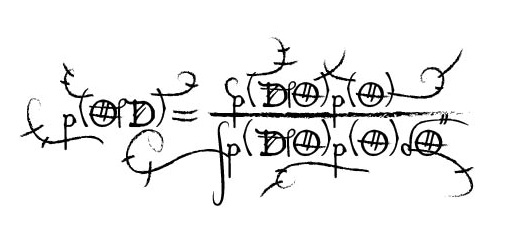
\includegraphics[width=1.5in]{Bayes.jpg}\hfil}\vfil}
%}

{
%\usebackgroundtemplate{\begin{center}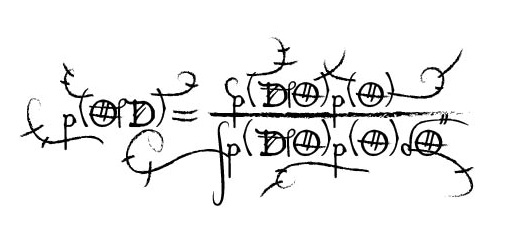
\includegraphics[width=0.4\paperwidth]{Bayes.jpg}\end{center}}
\usebackgroundtemplate{%
  \vbox to \paperheight{\hbox to \paperwidth{\hfil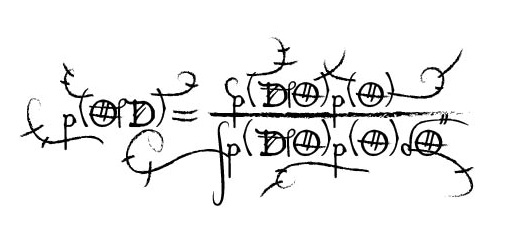
\includegraphics[width=2in]{Bayes.jpg}\hfil}}
}
\begin{frame}
\titlepage
\end{frame}
}
%\frame{\titlepage} 

%\frame{\frametitle{Overview of the talk}\tableofcontents}


\begin{frame}
\frametitle{Lecture overview}

\begin{itemize}
\item Markov processes
\bigskip
\item The concept of a stationary distribution of a Markov process
\bigskip
\item The Gibbs sampler
\bigskip
\item Data augmentation 
\begin{itemize}
\item Probit regression
\item Mixture models
\end{itemize}

\end{itemize}

\end{frame}


\frame{\frametitle{Markov processes}
\begin{itemize}
\item \textbf{For simplicity} consider a \textbf{\color{blue}discrete sample space} for $\theta$. \textbf{Example}:
\begin{equation*}
\pi(\theta) = \begin{cases}
1/4, &\text{if $\theta = \phi_1$,}\\
7/12, & \text{if $\theta = \phi_2$,} \\
1/6, & \text{if $\theta = \phi_3$.}
\end{cases}
\end{equation*}
\begin{definition}
A \textit{\color{blue}Markov} process is a collection of r.v's $\{\theta^{(t)}\}_{t\geq 0}$ with the property
$$\Pr(\theta^{(t)}=\phi^{(t)}|\theta^{(t-1)}=\phi^{(t-1)}, \dots, \theta^{(1)}=\phi^{(1)})=\Pr(\theta^{(t)}=\phi^{(t)} |\theta^{(t-1)}=\phi^{(t-1)}),$$
where $\phi^{(t)}$ denotes the state of the process at period $t$. \\
In the example with three states above: $\phi^{(t)}\in \{\phi_1, \phi_2, \phi_3\} \quad \forall t \geq 1$.
\end{definition}
\item A sequence generated by a Markov process is often called a \textbf{\color{blue}Markov chain}.
\item \textbf{\color{blue}Discrete state space} gives us a thorough intuition. \textbf{\textbf{\color{blue}}Continuous state space} is a generalization.
\end{itemize}
}


\begin{frame} %[fragile]
\frametitle{Transition probabilities}
\begin{center}
\begin{tikzpicture}[level 1/.style={sibling distance=3.5cm},
	level 2/.style={sibling distance=1cm}, node distance=2.5cm, ->, >=stealth']

	\tikzstyle{state}=[circle,thick,fill=blue!20,minimum size=8mm]   
	%\tikzstyle{empty}=[circle,draw=white!75,fill=white!20]  
	\node[state] (A) 	{$\phi_1$};
	\node[state] (B) [right of=A] {$\phi_2$};	
	\node[state] (C) [below of= A] {$\phi_3$};
	% From A to everyone	
	\path (A) edge  [bend left] node[above] {0.2} (B);
	\path (A) edge  [bend right] node[left] {0.3} (C);	
	\path (A) edge  [loop left] node[left] {0.5} (A);

	% From B to everyone	
	\path (B) edge  [bend left] node[above] {0.1} (A);
	\path (B) edge   node[right] {0.1} (C);		
	\path (B) edge  [loop right] node[right] {0.8} (B);

	% From C to everyone	
	\path (C) edge  [bend right] node[left] {0.4} (A);
	\path (C) edge  [loop left] node[left] {0.2} (C);
	\path (C) edge  [bend right] node[right] {0.4} (B);		
	%\path (B) edge   node[left] {0.1} (C);		
	%\path (B) edge  [loop above] node[above] {0.8} (B);

	%\path (A) edge  [bend right] node[left] {0.3} (C);	
	%

	%\path (A) edge  [bend right] node[below] {1} (B);
	%\path (B) edge  [bend right] node[above] {0.4} (A);
	%\begin{scope}
	%\node[state]{$\mu,\tau$}
	%	child{ node [state]{$\theta_1$}
	%	}
	%	child{ node [state]{$\theta_3$}
	%	}	
	%	;
	%\end{scope}

\end{tikzpicture}
\end{center}
\begin{itemize}
\item \textbf{\color{blue}Transition probabilities} and \textbf{\color{blue}transition matrix}: 
$$p_{ij} = \Pr(\theta^{(t)}=\phi_j|\theta^{(t-1)}=\phi_i) \quad  \text{and} \quad P=\{p_{ij}\} = \left[ \begin{matrix} 0.5&0.2&0.3\\ 0.1&0.8&0.1\\0.4&0.4&0.2 \end{matrix} \right] $$

\end{itemize}
%\begin{definition}
%The transition probability at period $j-1$, is the probability of 
%\end{definition}
\end{frame}


\frame{\frametitle{Simulating 100 draws from our process}

\begin{figure}[H]
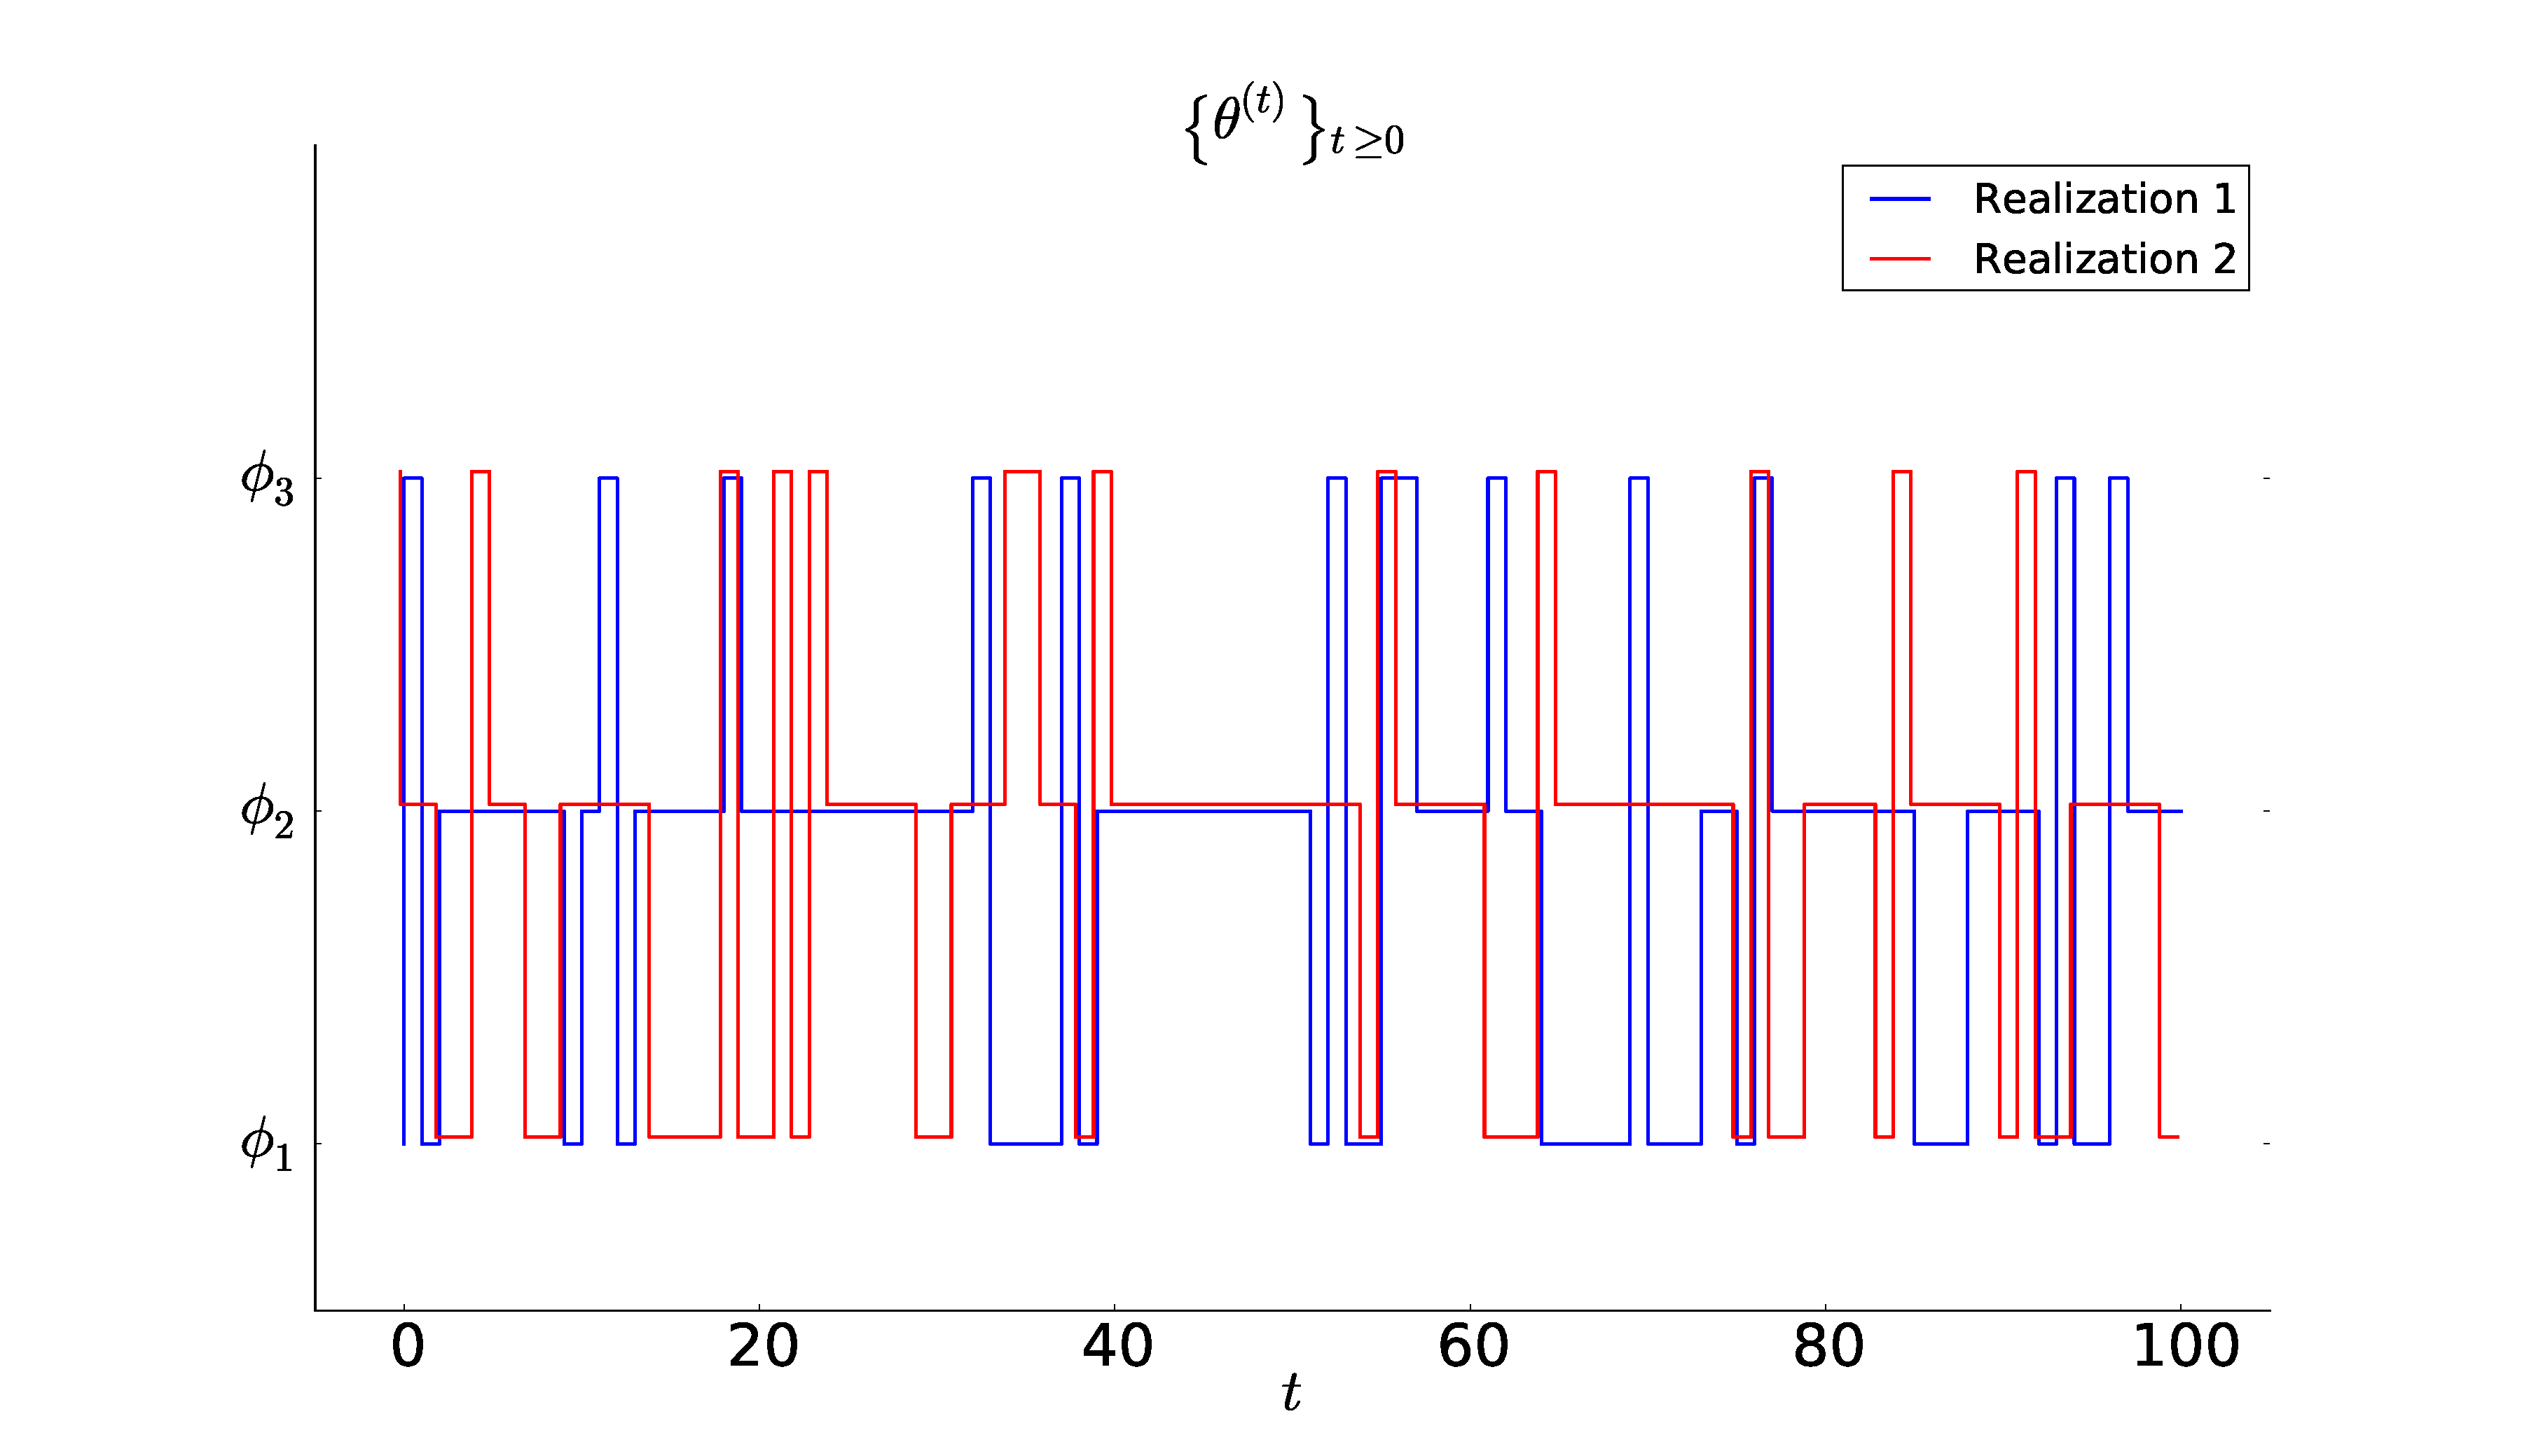
\includegraphics[width=\columnwidth]{markovchain}
%\protect\caption{$\p(\alpha, \beta|y)$}
\end{figure}
%\item \textbf{Homework:} Play with the code. \textbf{Make sure you understand} how to code the posterior {\color{blue}in logarithmic scale}. \textbf{\color{red}Extra:} Modify the code to handle more regressors (parameters). How many parameters are feasible?
}

\begin{frame} %[fragile]
\frametitle{Computing marginal distribution of the states at each $t$}
\begin{itemize}
\item \textbf{\color{blue}Marginal distribution} at time $t$
$$\pi^{(t)}_j = \Pr(\theta^{(t)}=\phi_j).$$
\item Let $\pi^{(0)}=(\pi^{(0)}_1, \pi^{(0)}_2, \pi^{(0)}_3)$ denote the \textbf{\color{blue}initial state distribution}, 
$$\pi^{(0)}_j = \Pr(\theta^{(0)}=\phi_j),$$i.e. the \textbf{\color{blue}marginal distribution} of state $j$ at $t=0$.
\item What is the \textbf{\color{blue}marginal distribution} in $t=1$ for state $j$?
$$\pi_j^{(1)}=\Pr(\theta^{(1)}=\phi_j)=\sum_i \underbrace{\Pr(\theta^{(1)}=\phi_j|\theta^{(0)}=\phi_i)}_{p_{ij}}\underbrace{\Pr(\theta^{(0)}=\phi_i)}_{\pi^{(0)}_i}.$$
\item In \textbf{matrix form} $\pi^{(1)}=\pi^{(0)} P$.


\end{itemize}

\end{frame}

\begin{frame} %[fragile]
\frametitle{Computing marginal distribution of the states  at each $t$, cont.}
\begin{itemize}
\item \textbf{What about} $\pi^{(2)}_j$?
\begin{eqnarray*}
\pi_j^{(2)} &=& \sum_i \sum_{i^{\prime}}\Pr(\theta^{(2)}=\phi_j|\theta^{(1)}=\phi_i, \theta^{(0)}=\phi_{i^{\prime}})\Pr(\theta^{(1)}=\phi_i, \theta^{(0)}=\phi_{i^{\prime}}) \\
~ & = & \sum_i \sum_{i^{\prime}}\underbrace{\Pr(\theta^{(2)}=\phi_j|\theta^{(1)}=\phi_i)}_{p_{ij}}\underbrace{\Pr(\theta^{(1)}=\phi_i | \theta^{(0)}=\phi_{i^{\prime}})}_{p_{i^{\prime}i}}\underbrace{\Pr( \theta^{(0)}=\phi_{i^{\prime}})}_{\pi_{i^{\prime}}^{(0)}} \\
~ & = & \sum_i  p_{ij}\underbrace{\sum_{i^{\prime}}p_{i^{\prime}i} \pi_{i^{\prime}}^{(0)}}_{\pi_i^{(1)}}.
\end{eqnarray*} 
\item \textbf{\color{blue}In fact}: $\pi^{(2)}=\pi^{(0)}P^2$ ($=\underbrace{\pi^{(0)}P}_{\pi^{(1)}}P=\pi^{(1)}P$).
\item \textbf{\color{blue}In general}: $\pi^{(n)}=\pi^{(0)}P^n$.

\end{itemize}

\end{frame}

\begin{frame} %[fragile]
\frametitle{Stationary distribution of the states}
\begin{itemize}
\item Suppose we observe the Markov process for an \textbf{\color{blue}infinite amount of time}.
\begin{enumerate}
\item Does the \textbf{\color{blue}marginal distribution} of the states ever \textbf{stabilize}? In other words
$$\lim_{t\rightarrow \infty} \pi^{(t)}=\pi\quad \text{ for some }\pi, \text{ regardless the initial } \pi^{(0)}?$$
\begin{figure}[H]
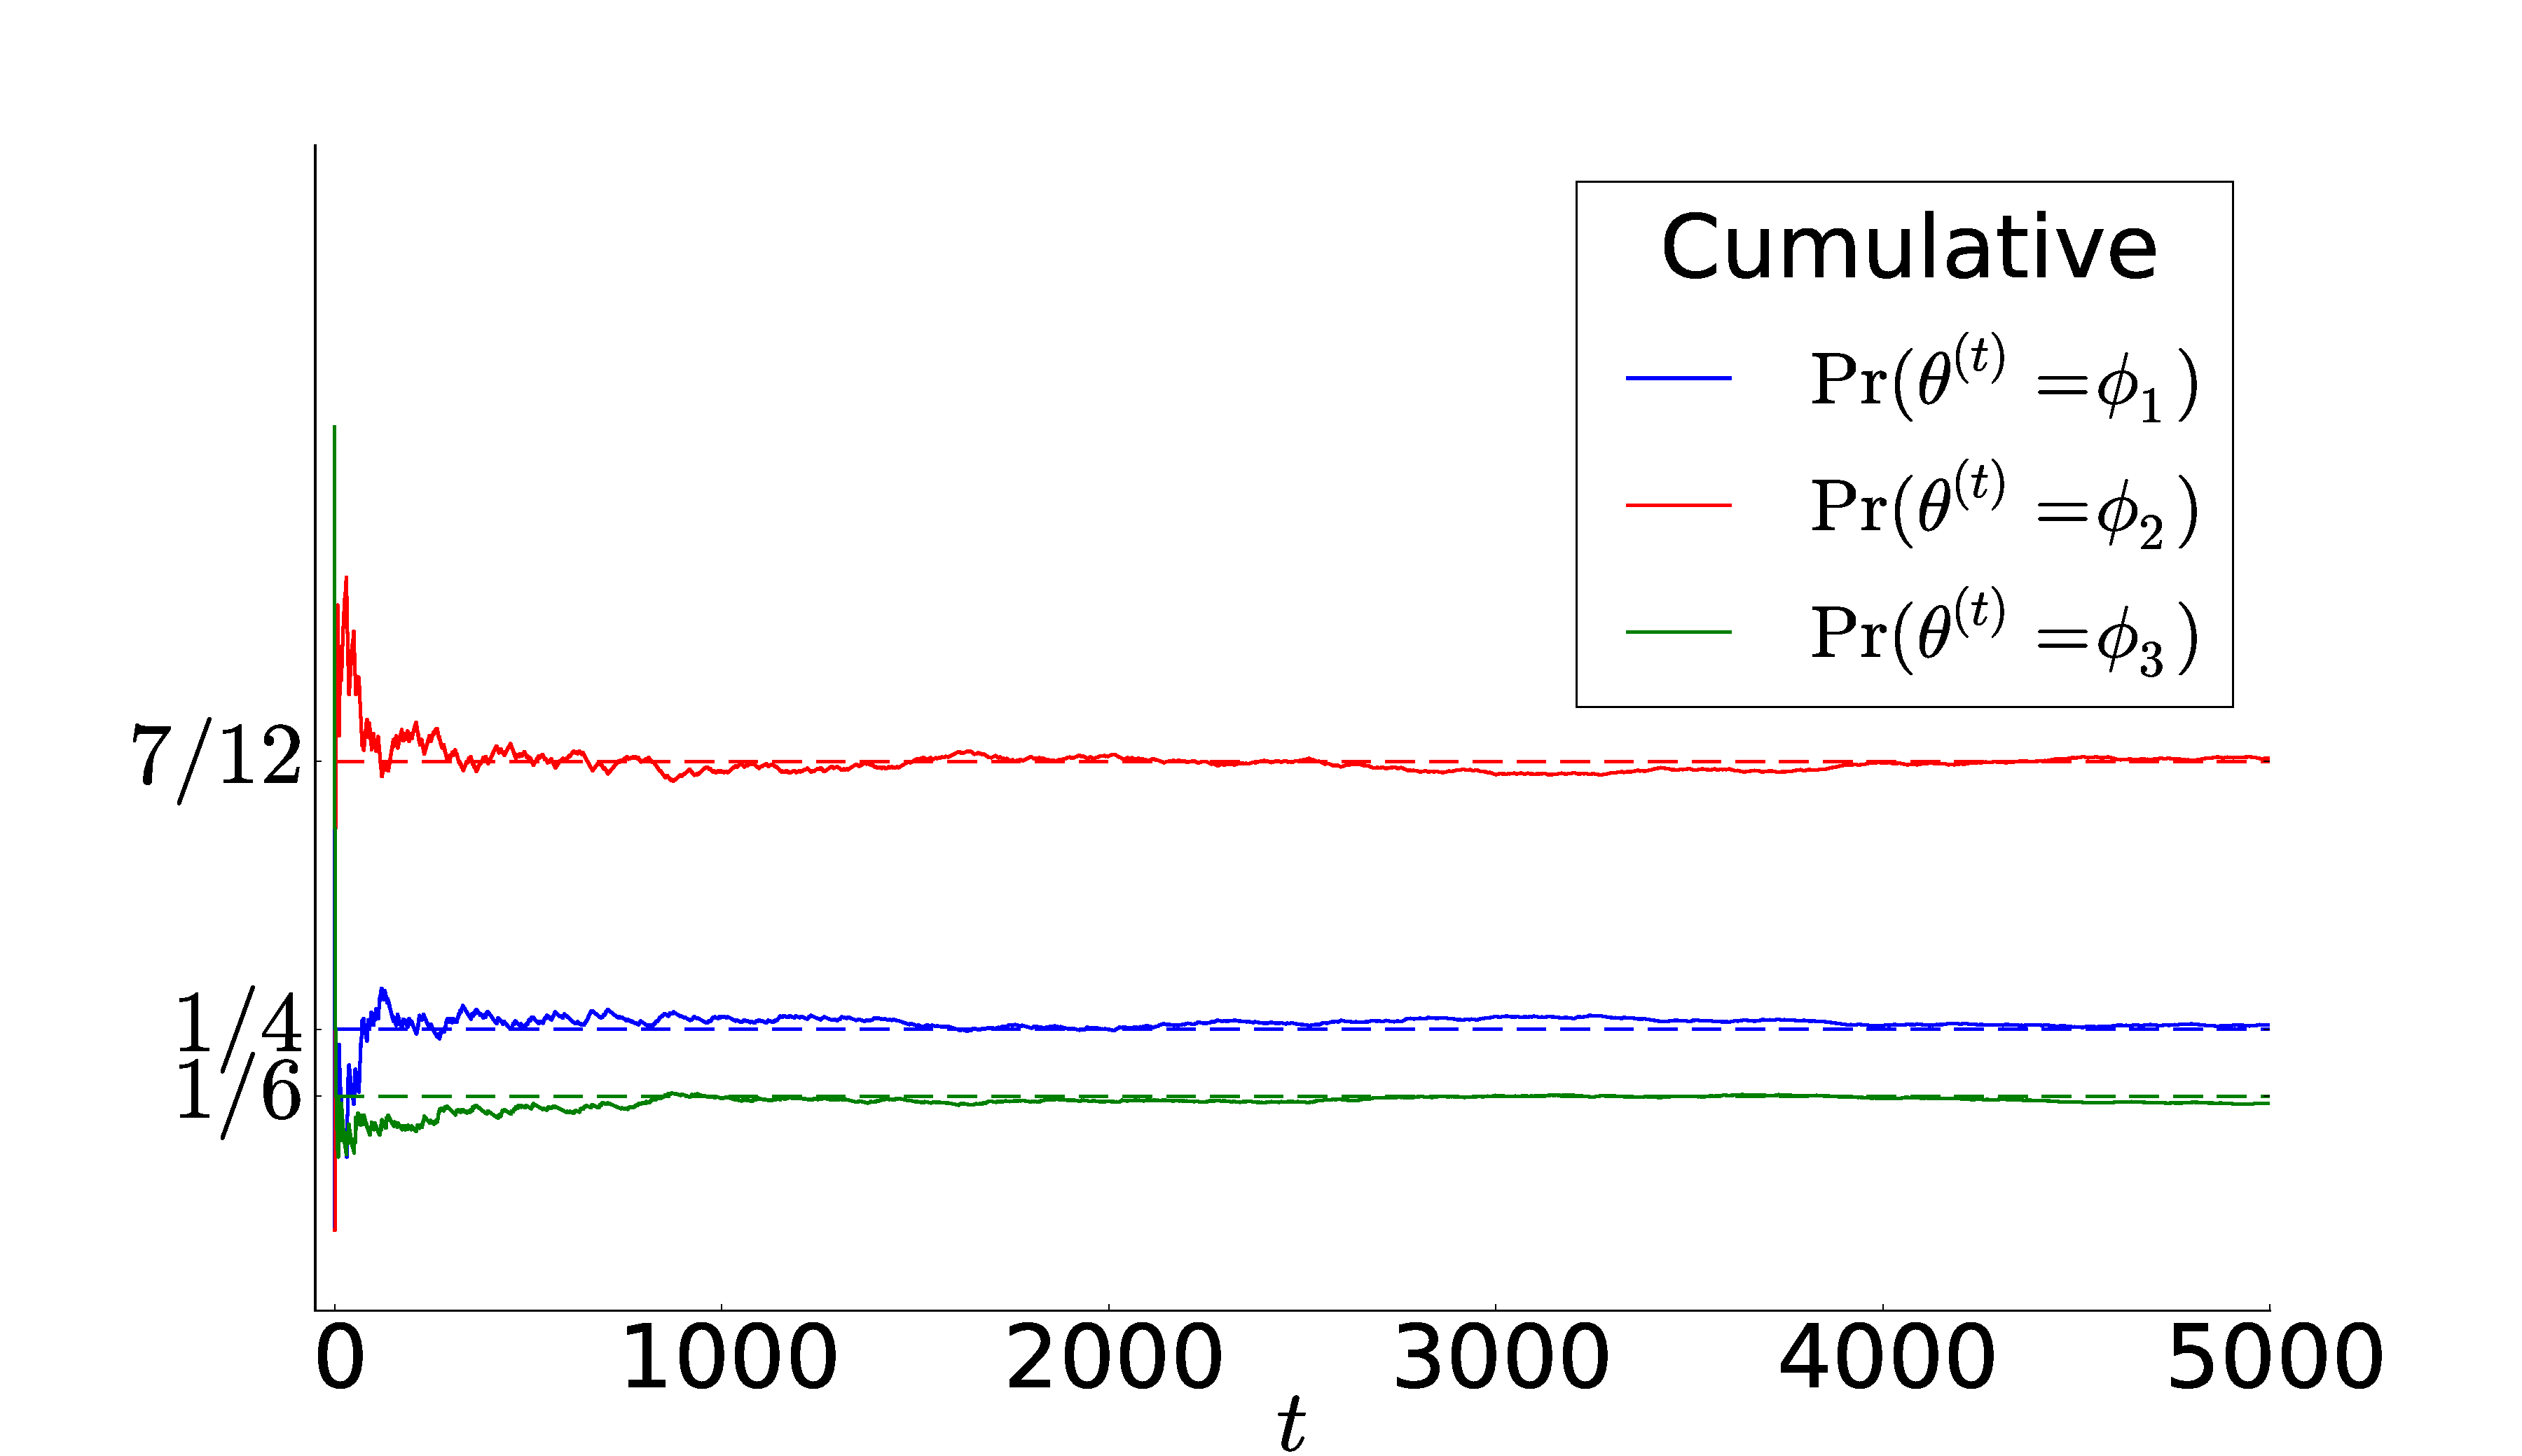
\includegraphics[width=0.45\columnwidth]{Cumulative1}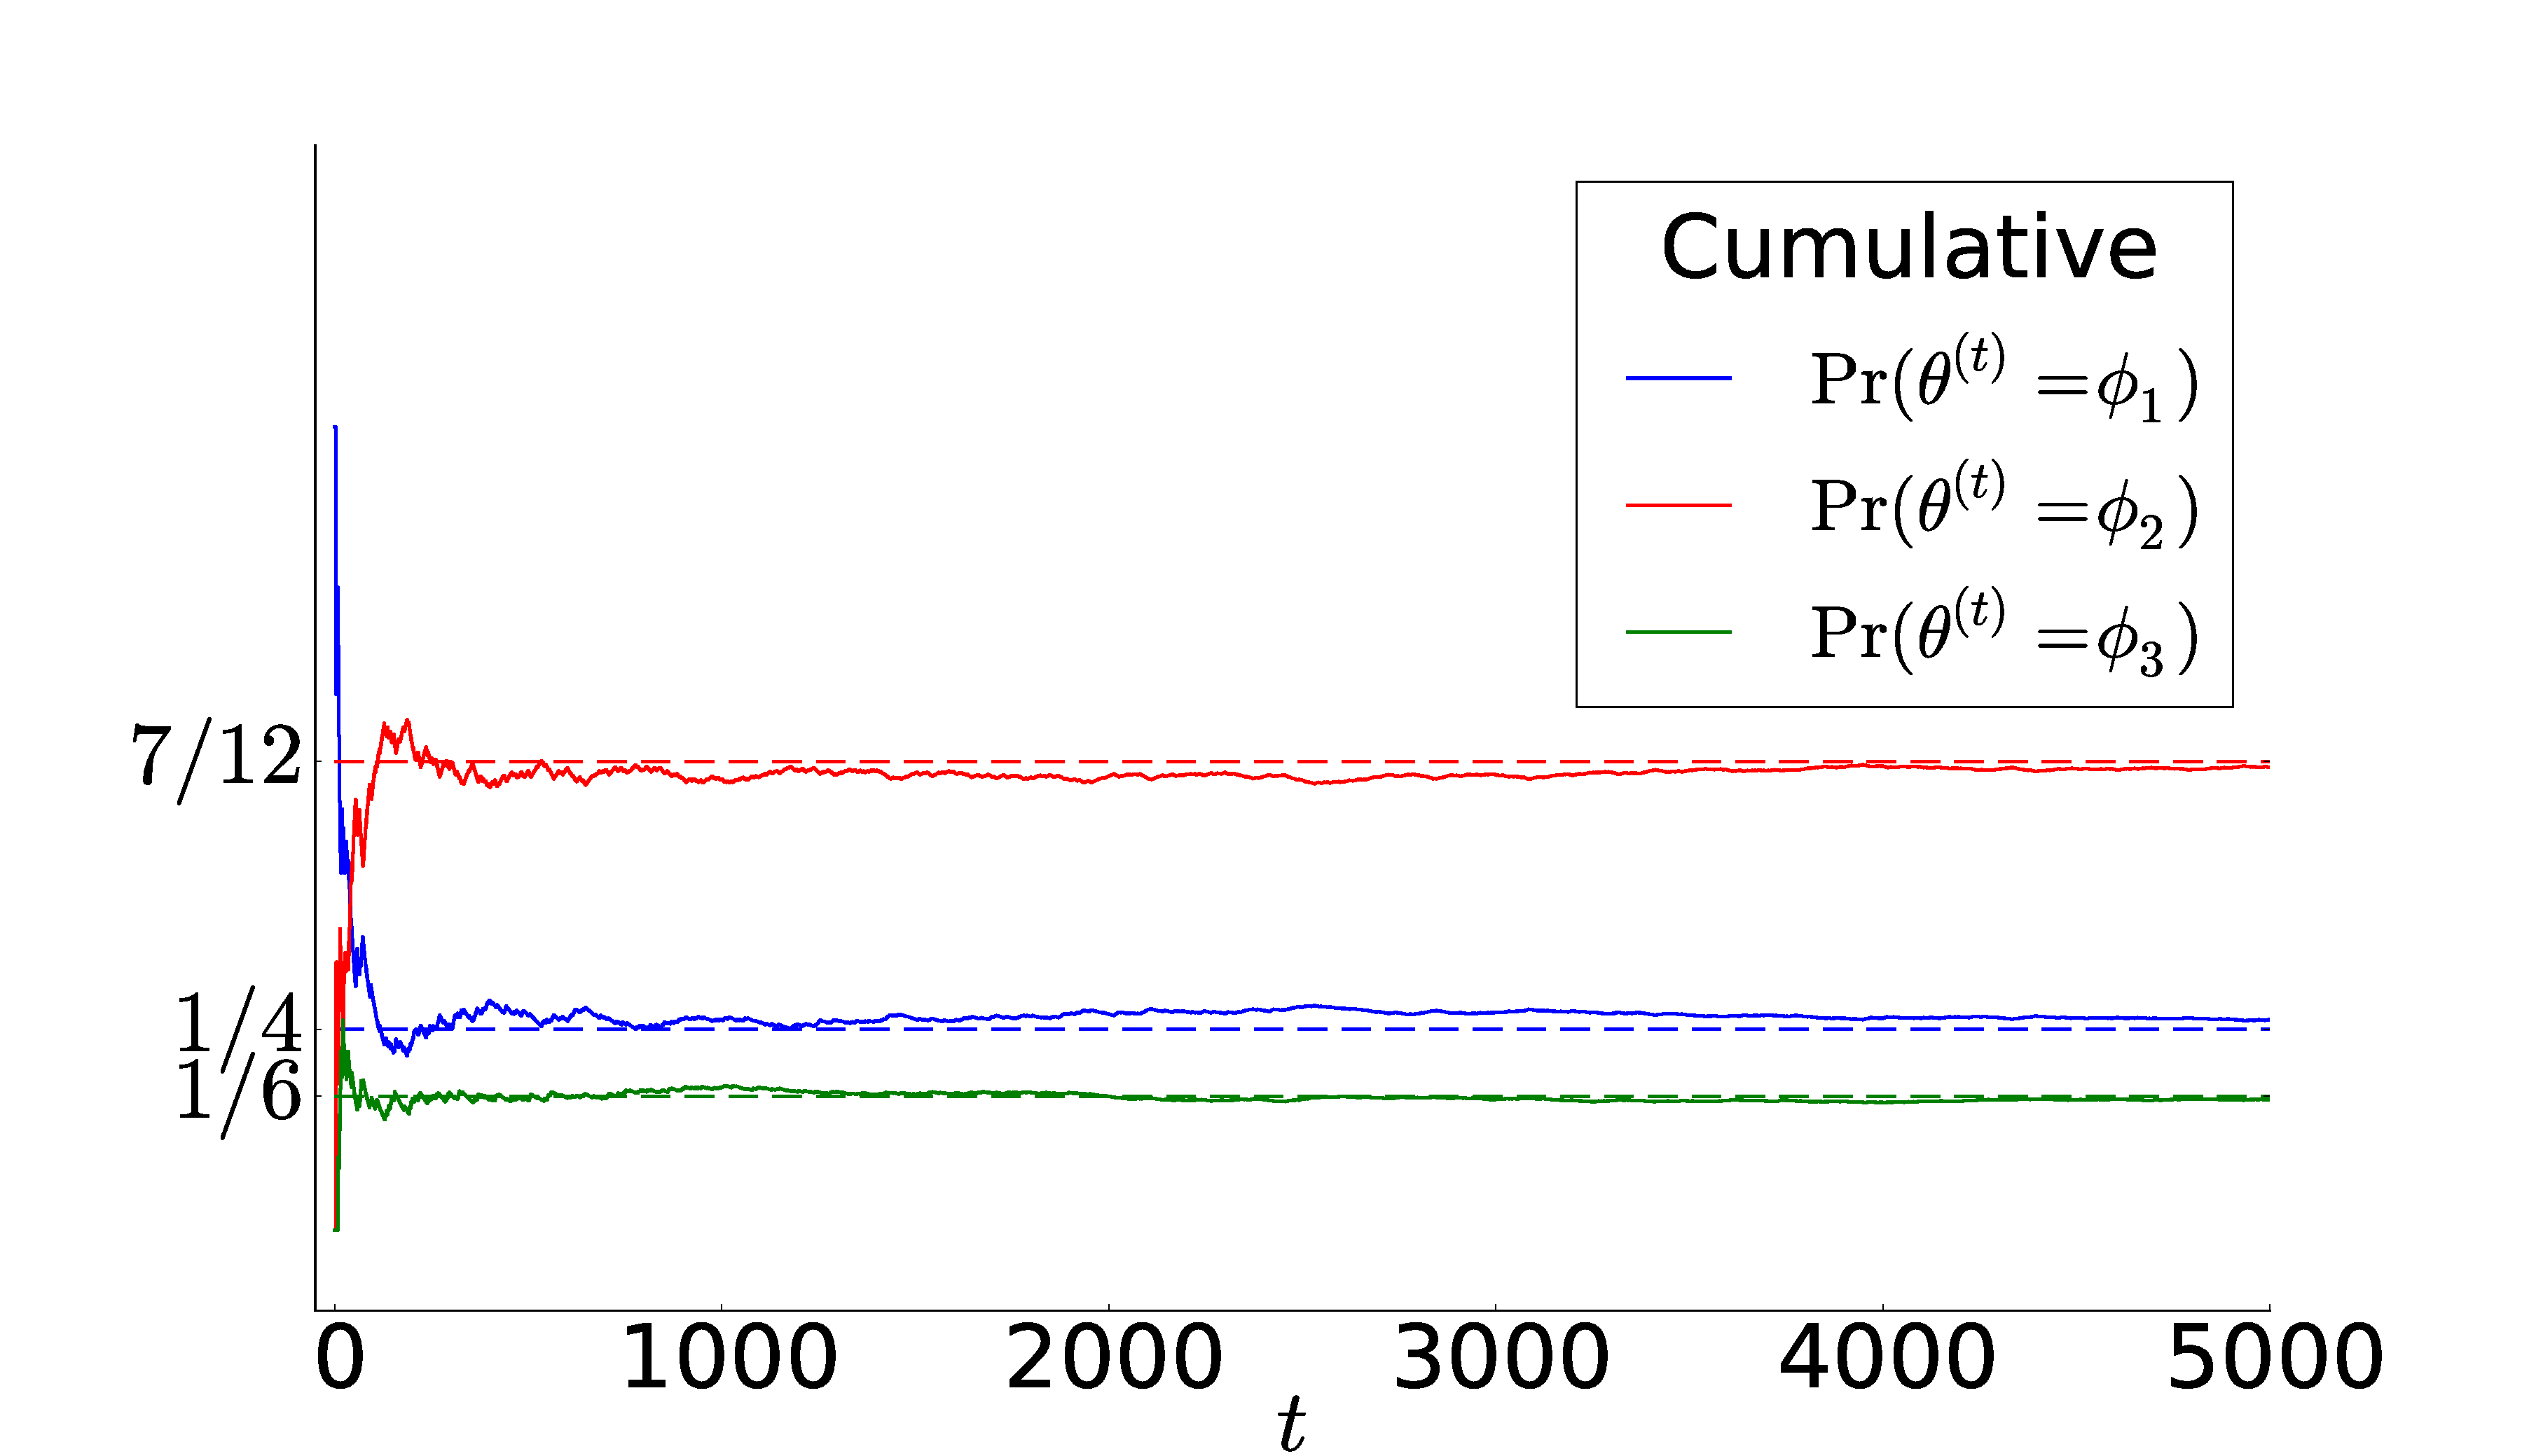
\includegraphics[width=0.45\columnwidth]{Cumulative2}
%\protect\caption{$\p(\alpha, \beta|y)$}
\end{figure}
\item Is $\pi$ \textbf{\color{blue}unique}?
\end{enumerate}

\end{itemize}
\end{frame}

\begin{frame} %[fragile]
\frametitle{Stationary distribution of the states, cont}
\begin{itemize}
\item \textbf{\color{blue}In fact} (under conditions {\color{blue}($*$)}, next slide), $$\lim_{t\rightarrow \infty}P^t = \mathbbm{1} \pi = \left[ \begin{matrix} \pi \\ \pi \\ \vdots \\ \pi \end{matrix}\right].$$
\item \textbf{\color{blue}The stationary distribution} $\pi$, such that $$\pi = \pi P,$$
\textbf{exists} and is \textbf{unique} under {\color{blue}($*$)}.



\end{itemize}

\end{frame}


\begin{frame} %[fragile]
\frametitle{Stationary distribution of the states, cont}
\begin{itemize}

\item[\color{blue}($*$)] \textbf{The Markov chain} must be: \begin{enumerate}
\item[(i)] \textbf{\color{blue}Irreducible}: \textbf{Positive probability} of reaching any state from any other state. \textbf{\color{red}Not true for}:
\begin{center}
\begin{tikzpicture}[level 1/.style={sibling distance=3.5cm},
	level 2/.style={sibling distance=1cm}, node distance=2.5cm, ->, >=stealth']

	\tikzstyle{state}=[circle,thick,fill=blue!20,minimum size=8mm]   
	%\tikzstyle{empty}=[circle,draw=white!75,fill=white!20]  
	\node[state] (A) 	{$\phi_1$};
	\node[state] (B) [right of=A] {$\phi_2$};	
	\node[state] (C) [right of=B] {$\phi_3$};
	% From A to everyone	
	\path (A) edge  [bend left] node[above] {0.2} (B);
	\path (A) edge  [loop left] node[left] {0.8} (A);

	% From B to everyone	
	\path (B) edge  [bend left] node[above] {0.5} (A);
	\path (B) edge   node[above] {0.5} (C);
	%\path (B) edge  [loop right] node[right] {1} (B);
	
	% From C
	\path (C) edge  [loop right] node[right] {1} (C);


\end{tikzpicture}
\end{center}
\item[(ii)] \textbf{\color{blue}Aperiodic}: Does \textbf{not} get into "predictable cycles". \textbf{\color{red}Predictable cycle}:
\begin{center}
\begin{tikzpicture}[level 1/.style={sibling distance=3.5cm},
	level 2/.style={sibling distance=1cm}, node distance=2.5cm, ->, >=stealth']

	\tikzstyle{state}=[circle,thick,fill=blue!20,minimum size=8mm]   
	%\tikzstyle{empty}=[circle,draw=white!75,fill=white!20]  
	\node[state] (A) 	{$\phi_1$};
	\node[state] (B) [right of=A] {$\phi_2$};	
	\node[state] (C) [right of=B] {$\phi_3$};
	% From A to everyone	
	\path (A) edge  node[above] {1} (B);

	% From B to everyone	
	\path (B) edge  node[above] {1} (C);
	%\path (B) edge  [loop right] node[right] {1} (B);
	
	% From C
	\path (C) edge [bend left] node[above] {1} (A);
	%\path (C) edge  [loop right] node[right] {1} (C);


\end{tikzpicture}
\end{center}
\item[(iii)] \textbf{\color{blue}Positive recurrent}: Expected time of returning to any state is \textbf{\color{red}finite}. Define $$T_i = \inf \{t\geq 1: \theta^{(t)}=\phi_i | \theta^{(0)}=\phi_i\}.$$
The condition is $$E[T_i] < \infty, \quad \text{for all states } i.$$ 
\end{enumerate}

\end{itemize}

\end{frame}

\begin{frame} %[fragile]
\frametitle{A sufficient condition to make life easier}
\begin{itemize}
\item Conditions 1-3 are \textbf{\color{red}necessary}. If true $\Rightarrow$ a unique stationary distribution.
\item There exist a \textbf{"stronger property"} - \textbf{\color{blue}reversible Markov chain}. Important for \textbf{\color{blue}Metropolis-Hastings} (makes life easier!) 
\begin{definition}
A \textbf{Markov chain} is \textbf{\color{blue}reversible} if there exist a distribution over the states, say $\pi$, such that
\begin{equation}
\label{eq:detailedbalance}
\Pr(\theta^{(t)}=\phi_j|\theta^{(t-1)}=\phi_i) \pi_i  = \Pr(\theta^{(t)}=\phi_i|\theta^{(t-1)}=\phi_j)  \pi_j,
\end{equation}
for all $t$ and all states $i$, $j$. Equation \eqref{eq:detailedbalance} is often called \textbf{\color{blue}the detailed balance condition}.
%$$\pi_i \Pr(\theta^{(t)}=\phi_j|\theta^{(t-1)}=\phi_i) = \pi_i \Pr(\theta^{(t)}=\phi_j|\theta^{(t-1)}=\phi_i)$$
\end{definition}
\item For a \textbf{\color{blue}reversible chain}, $\pi$ is always a \textbf{\color{blue}stationary distribution}:
{\small
\\$\Pr(\theta^{(t)}=\phi_j)=$
\begin{eqnarray*}
\sum_{i} \Pr(\theta^{(t)}=\phi_j|\theta^{(t-1)}=\phi_i)\pi_i  & \stackrel{\eqref{eq:detailedbalance}}{=}& \sum_{i} \Pr(\theta^{(t)}=\phi_i|\theta^{(t-1)}=\phi_j)\pi_j\\
~& = & \pi_j \overbrace{\sum_{i} \Pr(\theta^{(t)}=\phi_i|\theta^{(t-1)}=\phi_j)}^{=1 \text{ (probability)}} = \pi_j
\end{eqnarray*}}
\end{itemize}
\end{frame}

\begin{frame} %[fragile]
\frametitle{Understanding the reversibility condition in Eq. \eqref{eq:detailedbalance}}
\begin{itemize}
\item \textbf{Rewrite} Eq. \eqref{eq:detailedbalance} as 
\begin{eqnarray*}
\Pr(\theta^{(t)}=\phi_j|\theta^{(t-1)}=\phi_i) \pi_i & = & \Pr(\theta^{(t)}=\phi_i|\theta^{(t-1)}=\phi_j)  \pi_j \\
~ & \Leftrightarrow & ~ \\
\frac{\Pr(\theta^{(t)}=\phi_j,\theta^{(t-1)}=\phi_i)}{\Pr(\theta^{(t-1)}=\phi_i)} \pi_i & = & \frac{\Pr(\theta^{(t)}=\phi_i,\theta^{(t-1)}=\phi_j)}{\Pr(\theta^{(t-1)}=\phi_j)} \pi_j
\end{eqnarray*}
\item\textbf{ If we start the chain} at the stationary distribution $\pi$: 
$$\Pr(\theta^{(t)}=\phi_i)=\pi_i \quad \text{and} \quad \Pr(\theta^{(t)}=\phi_j)=\pi_j$$ 
for all $t$, thus {\color{blue}$\Pr(\theta^{(t)}=\phi_j,\theta^{(t-1)}=\phi_i)  =  \Pr(\theta^{(t)}=\phi_i,\theta^{(t-1)}=\phi_j)$}
%\begin{eqnarray*}
%\Pr(\theta^{(t)}=\phi_j,\theta^{(t-1)}=\phi_i) & = & \Pr(\theta^{(t)}=\phi_i,\theta^{(t-1)}=\phi_j).
%\end{eqnarray*}
\item \textbf{\color{blue}In words:} The (unconditional) probability of going from $\phi_i\rightarrow \phi_j$ is the same as going from $\phi_j \rightarrow \phi_i$. 
\item \textbf{"Stronger property"}: There are Markov chains that are \textbf{not} reversible but still have a stationary distribution. \textbf{Reversibility is a sufficient} (but \textbf{not} necessary) condition.
\end{itemize}
\end{frame}

\begin{frame} %[fragile]
\frametitle{Markov chains with continuous state space}
\begin{itemize}
\item \textbf{\color{blue}Transition kernel $T(\theta^{(t-1)}\rightarrow x)$} - a \textbf{conditional distribution} that expresses the probability to move to state $x$, \textbf{conditional} that the chain is at $\theta^{(t-1)}$. \medskip
%$$T(\theta^{(t-1)}\rightarrow \theta^{(t)})= \text{(Conditional) distribution of a move between } t-1 \text{ and } t$$
\item In \textbf{dicrete and finite state space} (what we have seen so far)
$$T_{ij}(\theta^{(t-1)}\rightarrow \theta^{(t)})= \Pr(\theta^{(t)}=\phi_j|\theta^{(t-1)}=\phi_i)$$\medskip
\item In \textbf{continuous state space}
$$T(\theta^{(t-1)}\rightarrow d\theta^{(t)})= \Pr(d\theta^{(t)}|\theta^{(t-1)})$$\medskip
\item $d\theta^{(t)}=\text{Region in }\theta \text{ space}$.\medskip
%\item Note that $T(\theta^{(t-1)}\rightarrow \mathbb{R})=1$. Since it is a distribution function
\item \textbf{Example (next lecture):}
The \textbf{\color{blue}Metropolis-Hastings algorithm} uses the \textit{detailed balance condition} to determine $T$. By construction this gives a chain that converges to $\pi(\theta)=p(\theta|y)$.

\end{itemize}
\end{frame}


\begin{frame} %[fragile]
\frametitle{Computing expectations of a function using dependent draws}
\begin{itemize}
\item \textbf{\color{blue}Recall:} we use the draws to estimate $I=E[h(\theta)]=\int h(\theta)\pi(\theta)d\theta$ by
$$\hat{I} = \frac{1}{N}\sum_{i=1}^N h(\theta^{(i)})$$
\item The draws are \textbf{(Markov) dependent}... will it still work?
\item \textbf{Yes}, in fact
$$\hat{I} = \frac{1}{N}\sum_{i=1}^N h(\theta^{(i)}) \xrightarrow{a.s} E[h(\theta)]$$
still holds!
\item The \textbf{statistical efficiency} of $\hat{I}$ is \textbf{\color{red}reduced} because of the dependence.
\item We have sacrificed the iid property and get \textbf{\color{red}less efficient draws}. \textbf{\color{blue}In exchange}: we can handle \textbf{larger} dimensions of $\theta$.
\end{itemize}
\end{frame}




\begin{frame}
\frametitle{The Gibbs sampler}
\begin{itemize}
\item Suppose the parameter vector is divided into $K$ \textbf{blocks}
$$\theta = (\theta_1, \dots, \theta_K).$$
\item Each $\theta_k$, $1\leq k \leq K$ can be either a scalar or a vector itself.
\item The Gibbs sampler is convenient when $$\pi(\theta)=\pi(\theta_1, \dots, \theta_K)\quad[ = p(\theta_1, \dots, \theta_K |y)]$$ is \textbf{difficult to simulate}, but it is \textbf{\color{red}easy to simulate} the \textbf{\color{blue}full conditional posteriors}
$$\pi(\theta_1|\theta_2, \theta_3 \dots, \theta_K)$$
$$\pi(\theta_2|\theta_1, \theta_3 \dots, \theta_K)$$
$$\vdots$$
$$\pi(\theta_K|\theta_1, \theta_2, \dots, \theta_{K-1})$$
\item \textbf{\color{blue}The Gibbs sampler} simulates from $\pi(\theta)$ by \textbf{alternating} the \textbf{\color{blue}full conditionals}.
\end{itemize}
\end{frame}

\begin{frame}
\frametitle{The Gibbs sampler, cont.}
\begin{center}
\begin{minipage}{\columnwidth}
\begin{varblock}[0.8\columnwidth]{The Gibbs sampler}
Obtain $N$ samples from $\pi(\theta)$.
\begin{itemize}
\item Set an (arbitrary) start point $$\theta^{(0)}=(\theta_1^{(0)},\theta_2^{(0)}, \dots,\theta_K^{(0)}).$$
\item \textbf{For} $i=1,\dots, N$, \textbf{repeat}
\end{itemize}
\begin{enumerate}
\item $\theta_1^{(i)} \sim \pi(\theta_1|\theta_2^{(i-1)}, \theta_3^{(i-1)}, \dots,\theta_K^{(i-1)})$,
\item $\theta_2^{(i)} \sim \pi(\theta_2|\theta_1^{(i)},\theta_3^{(i-1)}, \dots
\theta_K^{(i-1)})$,
\item[] $\phantom{\theta_1^{(i)}..} \vdots$
\item[K.] $\theta_K^{(i)} \sim \pi(\theta_K|\theta_1^{(i)}, \theta_2^{(i)}, \dots,\theta_{K-1}^{(i)})$.
\end{enumerate}
\end{varblock}
\end{minipage}
\end{center}
\begin{itemize}
\item \textbf{\color{blue}Note}: in each draw, the \textbf{latest update} of each block is used.
\end{itemize}

\end{frame}

\begin{frame}
\frametitle{Example: Simulating a bivariate Normal distribution}
\begin{itemize}
\item \textbf{\color{red}Note:} This examples is only for \textbf{illustration purposes}. There are \textbf{much more} efficient non-Markovian algorithms to do this.
\item \textbf{Bivariate normal}
$$\theta =\left[\begin{matrix}
 \theta_1 \\ \theta_2
\end{matrix}\right] \sim \mathcal{N}\left( \left[\begin{matrix} \mu_1 \\ \mu_2 \end{matrix}\right], \left[\begin{matrix} \sigma^2_1 & \rho \sigma_1\sigma_2 \\ \rho \sigma_2\sigma_1  & \sigma^2_2 \end{matrix}\right] \right)$$ 
\item \textbf{The full conditionals} (standard result for normal variates).
\begin{eqnarray*}
\theta_1 | \theta_2 & \sim & \mathcal{N}\left(\mu_1 + \rho \frac{\sigma_1}{\sigma_2}(\theta_2-\mu_2), (1-\rho^2)\sigma^2_1\right) \\ 
\theta_2 | \theta_1 & \sim & \mathcal{N}\left(\mu_2 + \rho \frac{\sigma_2}{\sigma_1}(\theta_1-\mu_1), (1-\rho^2)\sigma^2_2\right).
\end{eqnarray*}
\item Illustration (next slide) with $$\mu_1 = \mu_2 = 0, \quad \sigma^2_1 = \sigma^2_2 = 1 \quad \text{and} \quad \rho = 0.5$$
\item \textbf{Note:} The order of the full conditionals \textbf{does not matter}. 
\end{itemize}
\end{frame}

\begin{frame}
\frametitle{Example: Simulating a bivariate Normal distribution, cont}
\begin{figure}[H]
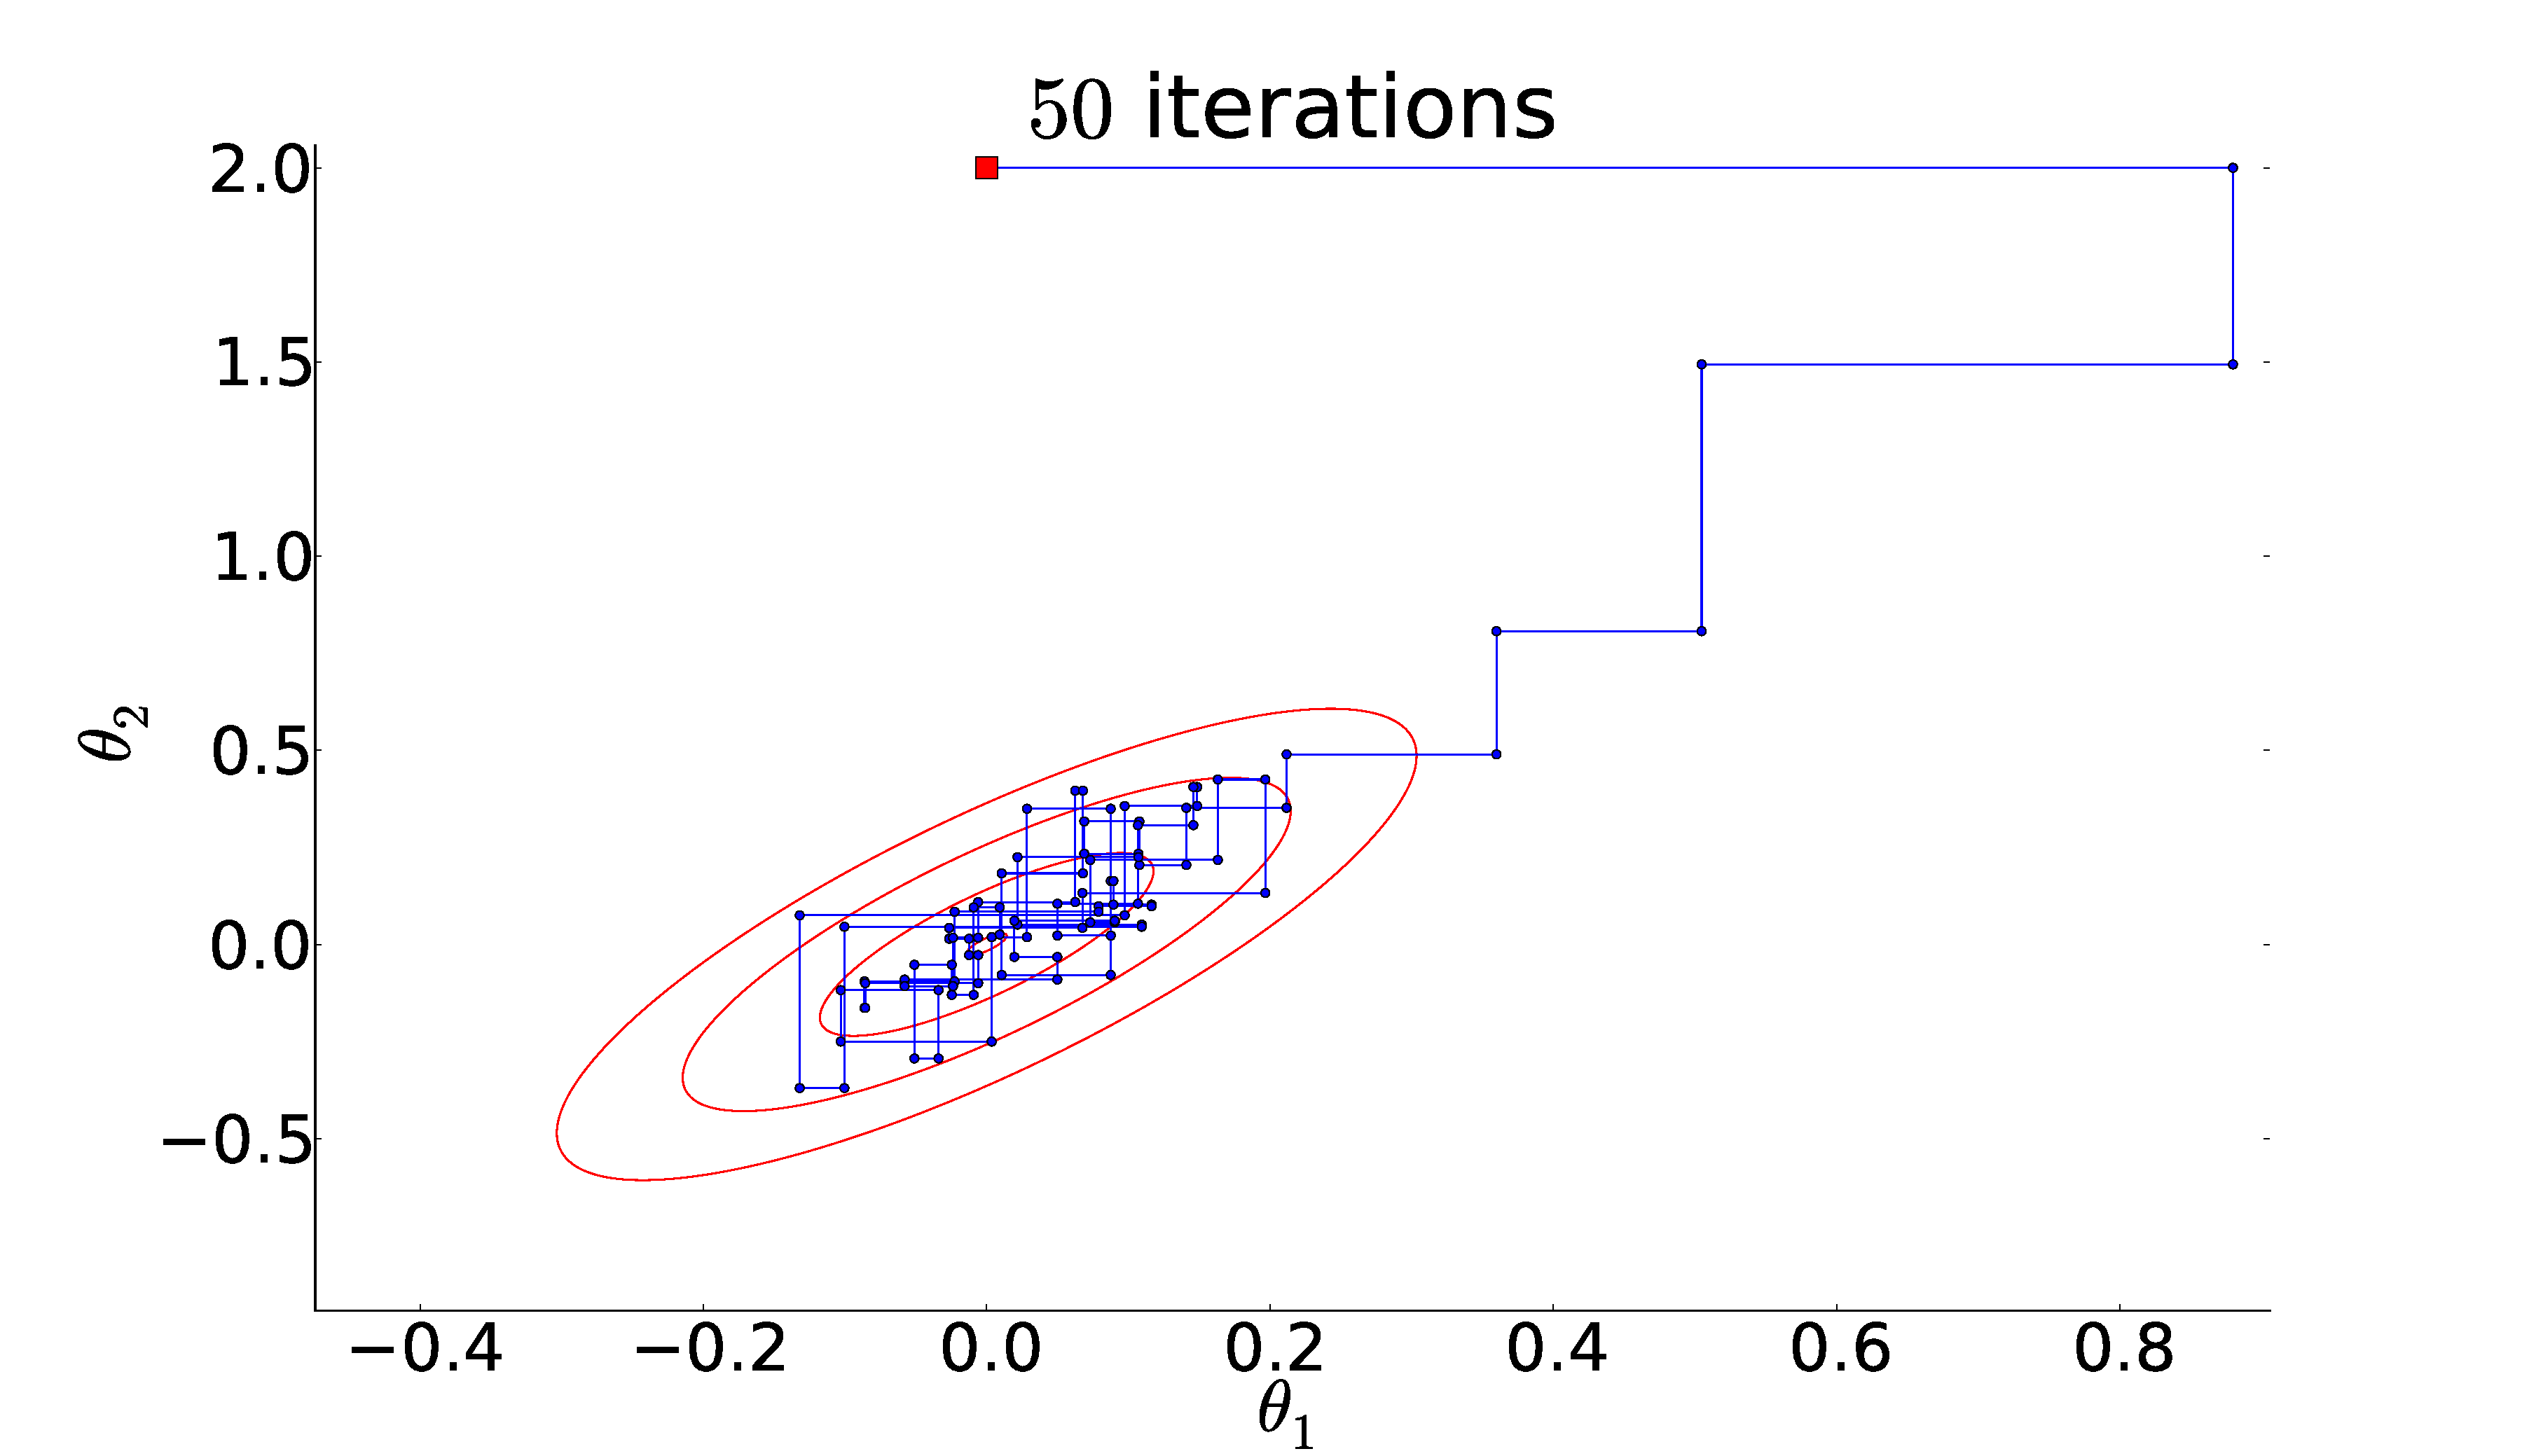
\includegraphics[width=0.5\columnwidth]{GibbsNormal50} 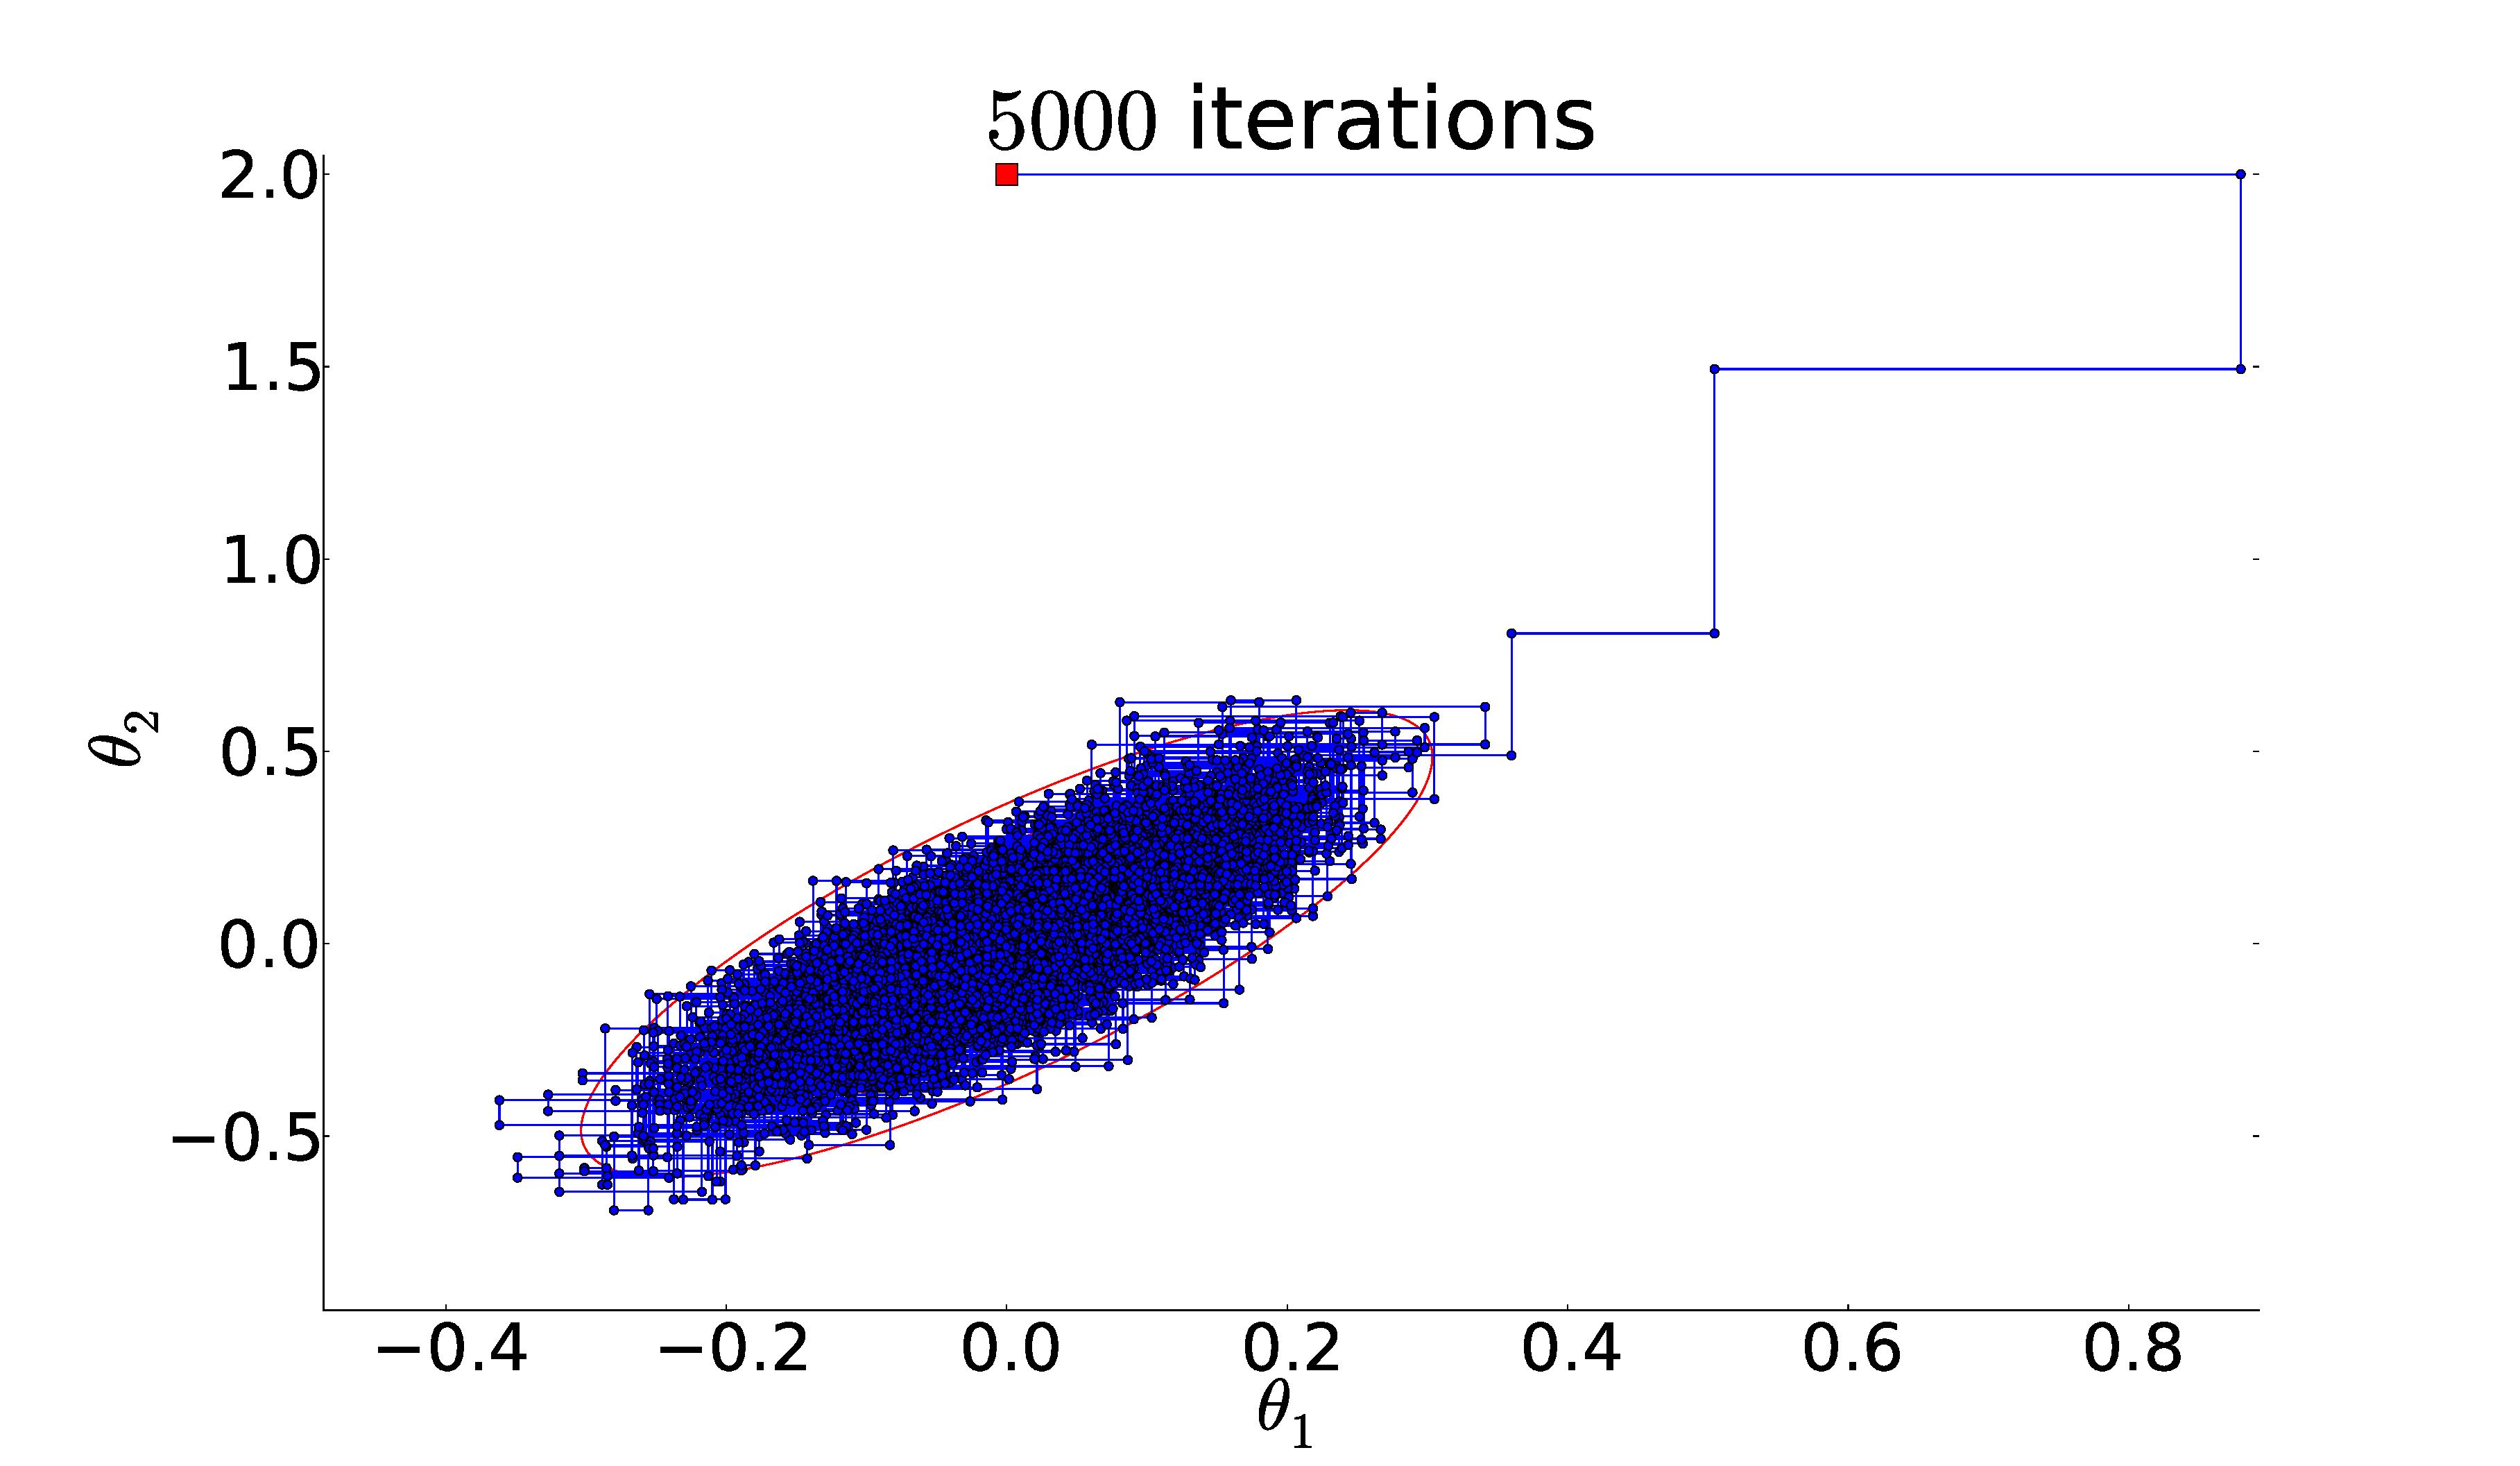
\includegraphics[width=0.5\columnwidth]{GibbsNormal5000}
%\protect\caption{$\p(\alpha, \beta|y)$}
\end{figure}
\begin{itemize}
\item The \textbf{contour plots} is the true $\pi(\theta_1, \theta_2)$.
\item The \textbf{blue dots} are samples from $\pi(\theta_1, \theta_2)$ (after burn-in).
\item Interested in the marginal of $\theta_1$?. The \textbf{\color{blue}histogram} or \textbf{\color{blue}kernel density} of $\theta_1$ approximates $\pi(\theta_1)$.
\item The chain \textbf{"forgets"} the initial state.
\end{itemize}
\end{frame}


\begin{frame}
\frametitle{Efficiency of the simulation}
\begin{itemize}
\item We compare to \textbf{\color{blue}direct} simulation, where $\theta_1, \theta_2$ are sampled jointly from a bivariate normal (and not dependent on previous draws). \textbf{\color{red}More on measures of efficiency later}.
\end{itemize}
\begin{figure}[H]
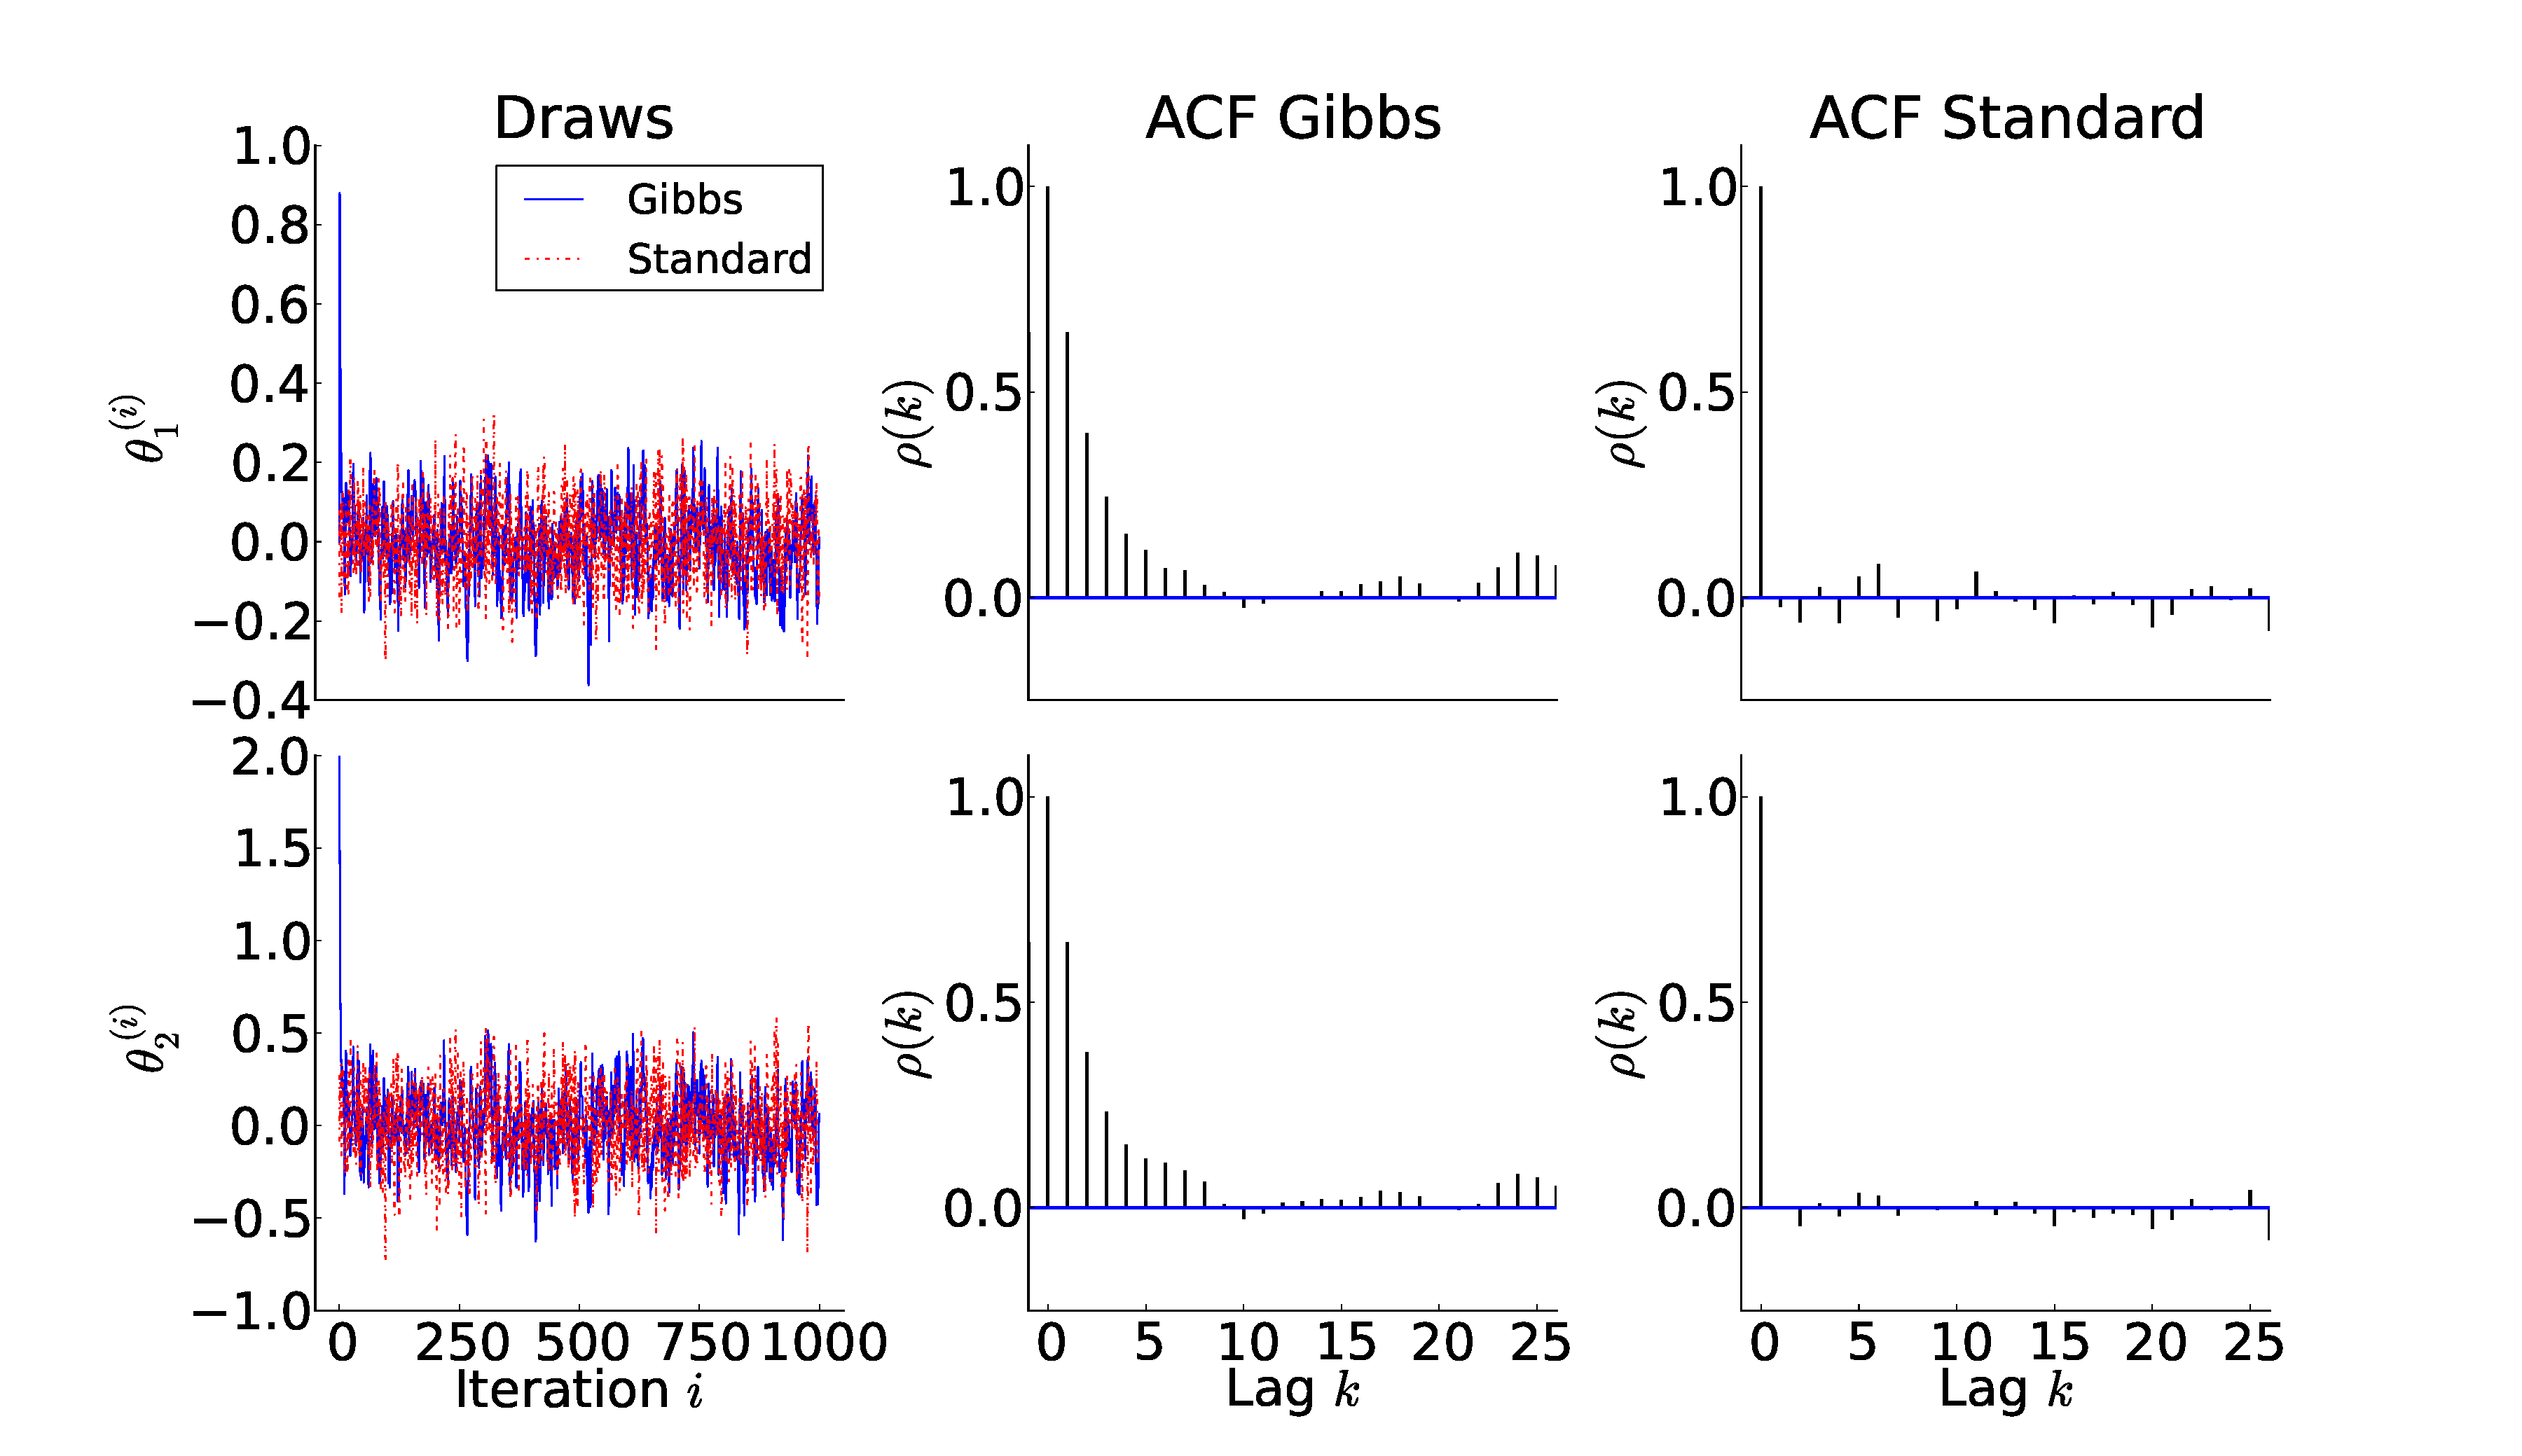
\includegraphics[width=\columnwidth]{GibbsNormalEfficiency}
%\protect\caption{$\p(\alpha, \beta|y)$}
\end{figure}

\end{frame}
%
%\begin{frame}
%\frametitle{Efficiency of the simulation, cont.}
%\begin{itemize}
%\item If $\theta_1$ and $\theta_2$ are very correlated the Gibbs sampler will be inefficient. Takes a lot of time to explore the distribution.
%\item Correlated parameters should be included in the same block.
%\item A re-parametrization of the model can improve the sampler.
%\item If parameters are correlated augmenting the model with more parameters can break the dependence and give a more efficient sampler. 
%\end{itemize}
%
%\end{frame}
%

\begin{frame}
\frametitle{The power of Gibbs... and its drawback}
\begin{itemize}
\item \textbf{\color{blue}Pros}:
\begin{itemize}
\item Makes many hierarchical models a \textbf{\color{blue}piece of cake} to estimate.
\item \textbf{\color{blue}Data augmentation} - very powerful tool.
\item Appealing treatment of \textbf{\color{blue}missing data} problems.
\end{itemize}
\bigskip
\item \textbf{\color{red}Cons}:
\begin{itemize}
\item \textbf{\color{blue}Inefficient if the blocks are correlated}. Takes a lot of time (\textbf{many draws}) to explore the posterior distribution.
\end{itemize}
\end{itemize}
\bigskip

\begin{itemize}
\item \textbf{Fighting} the \textbf{\color{red}cons}:
\begin{enumerate}
\item \textbf{\color{blue}Heavily correlated parameters} should always be included \textbf{in the same block}.
\item A \textbf{\color{blue}re-parametrization} of the model can improve the efficiency.
\item Introducing \textbf{\color{blue}extra parameters} in your model can \textbf{break} the correlation.
\end{enumerate}
\end{itemize}


\end{frame}

\begin{frame}
\frametitle{Gibbs sampling - the general strategy}
\begin{itemize}
\item \textbf{Notation}: $\theta_{\neg k} = \text{all blocks {\color{blue}except} the }k\text{th}$.\bigskip
\item The \textbf{\color{blue}full conditional} of any block $k$ is proportional to the \textbf{likelihood times the prior}:
\begin{eqnarray*}
\pi(\theta_k|\theta_{\neg k})  & = & \frac{p(\theta,y)}{p(\theta_{\neg k},y)} \\
~  & \propto & p(\theta|y) \propto p(y|\theta)p(\theta),
\end{eqnarray*}
where $\theta = (\theta_1,\dots,\theta_K)$.\bigskip
\item \textbf{\color{blue}Strategy to derive the full conditional for} $\theta_k$: throw away \textbf{\color{red}everything that does not depend on }$\theta_k$ in $p(y|\theta)p(\theta)$. Choose a \textbf{\color{blue}conjugate prior} for the $k$th block ($\theta_k$) if possible.
%\item \textbf{Example}: \textbf{\color{blue}Hierarchical normal} from lecture 1 revisited. No simplified version, assume \textbf{all parameters} are unknown.
\end{itemize}
\end{frame}
%
%
%\begin{frame}
%\frametitle{Data augmentation and the Gibbs sampler}
%\begin{itemize}
%\item Introducing \textbf{auxiliary variables} (data augmentation) can simplify estimation. \textbf{\color{blue}Example:} Finite mixture of normals.
%\item Let $M$ be the number of \textbf{components} and let $$\mu = (\mu_1, \dots, \mu_M)^{\prime} \quad  \sigma^2 = (\sigma^2_1, \dots, \sigma^2_M)^{\prime} \quad \text{and} \quad \omega = (\omega_1, \dots, \omega_M)^{\prime}.$$
%\item The model
%\begin{eqnarray*}
%y_i | \mu, \sigma, \omega & \sim & \sum_{m=1}^M \omega_m \mathcal{N}(\mu_m, \sigma^2_m), \quad \sum_{m=1}^M \omega_m = 1
%\end{eqnarray*}
%%\item This model can be very flexible
%\begin{figure}[H]
%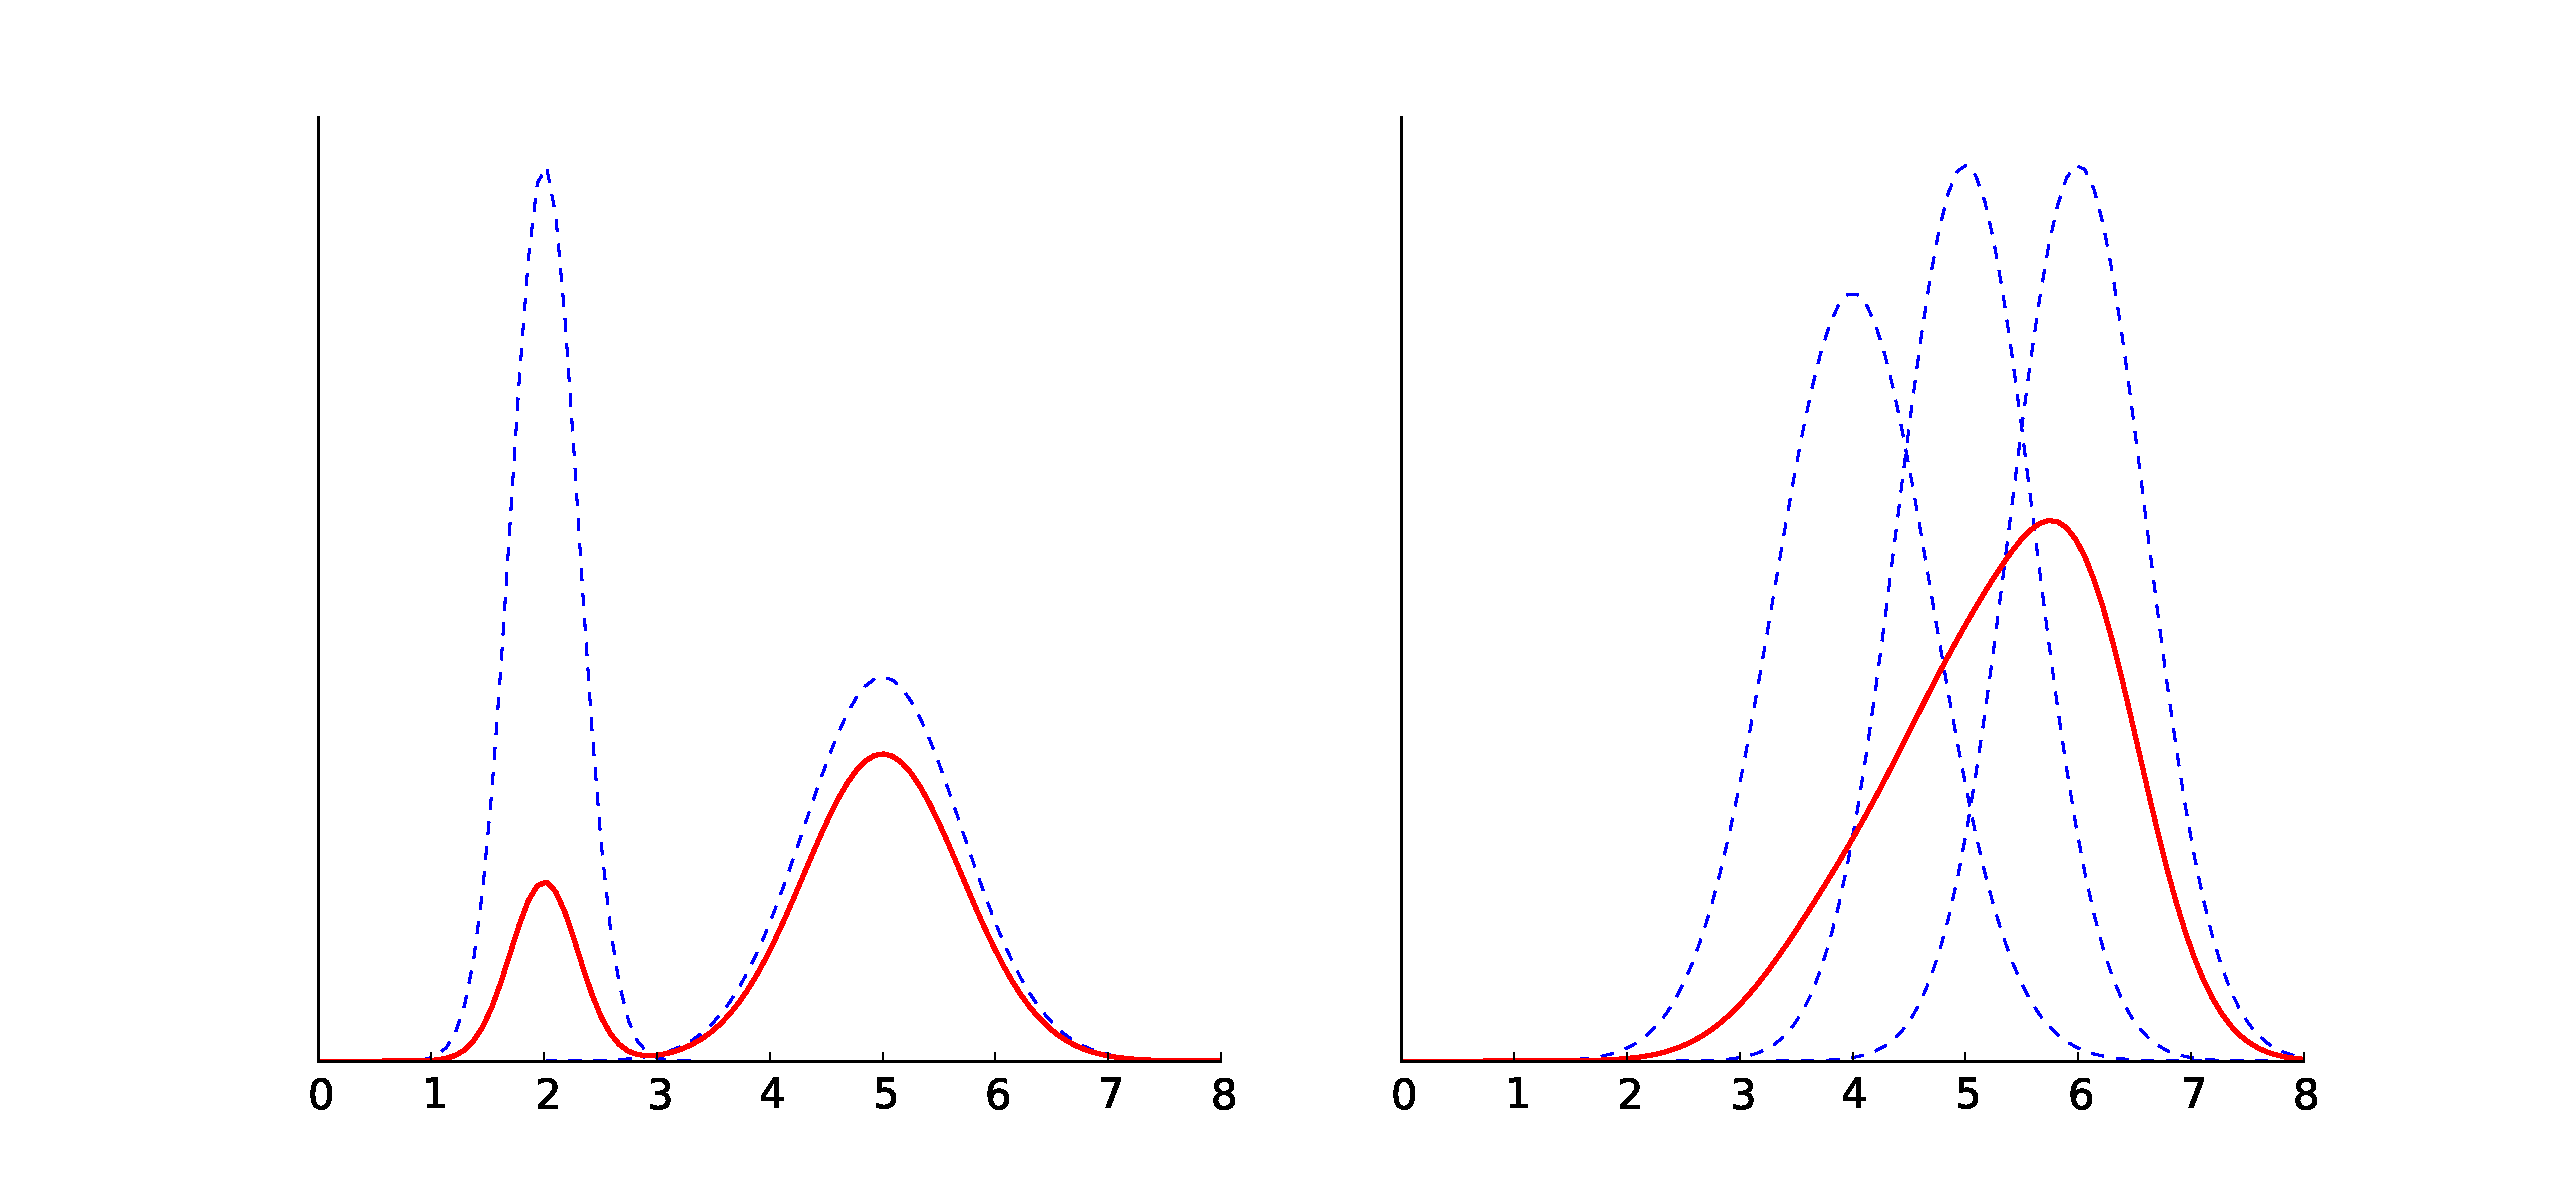
\includegraphics[width=0.5\columnwidth]{FiniteMixture}
%\protect\caption{Finite mixture of Gaussians (components in blue). Modeling a bimodal distribution (left) with M=2 and a skewed distribution (right) with M=3.}
%\end{figure}
%\end{itemize}
%\end{frame}
%
%\begin{frame}
%\frametitle{Finite Mixture of normals and data augmentation}
%\begin{itemize}
%\item The posterior is a \textbf{headache}
%$$\pi(\theta)=p(\mu, \sigma^2,\omega|y) \propto \overbrace{\left(\prod_{i=1}^n \left( \sum_{m=1}^M \omega_m \mathcal{N}(y_i|\mu_m, \sigma^2_m)\right)\right)}^{p(y|\mu, \sigma^2,\omega)}p(\mu, \sigma^2, \omega).$$
%\item \textbf{Data augmentation}: Let $s_i$ denote the \textbf{component membership} of the $i$th observation. 
%\item \textbf{Alternative} formulation of the model
%\begin{eqnarray*}
%y_i |\mu_m , \sigma^2_m, s_i = m &\sim & \mathcal{N}(\mu_m, \sigma^2_m) \\
%\Pr(s_i = m|\omega_m) & = & \omega_m,
%\end{eqnarray*}
%\item If we knew $s_i$ life is easy because the model \textbf{\color{blue}is just Gaussian}...
%
%%\item \textbf{If we knew} that observation $i$ was generated from the $m$th component, then
%%\begin{eqnarray*}
%%y_i |\mu_m , \sigma^2_m, s_i = m &\sim & \mathcal{N}(\mu_m, \sigma^2_m) \\
%%\Pr(s_i = m|\omega_m) & = & \omega_m,
%%\end{eqnarray*}
%%is an alternative formulation of the model.
%\item But \textbf{we don't know} $s$... \pause \textbf{Gibbs sampling!:} Initialize $s$ randomly and \textbf{update all parameters}. Given all the parameters \textbf{update $s$}... and so on.
%\item We have \textbf{augmented} the model \textbf{with artificial data} $s=(s_1,\dots,s_n)$. \textbf{\color{blue}Data augmentation}.
%\end{itemize}
%\end{frame}
%
%\begin{frame}
%\frametitle{Finite Mixture of normals and data augmentation, cont}
%\begin{itemize}
%\item The \textbf{augmented} posterior 
%\begin{eqnarray*}
%p(\mu,\sigma^2, s, \omega|y) & \propto & p(y|\mu,\sigma^2,s,\omega)p(\mu,\sigma^2,s,\omega) \\
%~ & = & p(y|\mu,\sigma^2,s)p(\mu,\sigma^2)p(s|\omega)p(\omega) \\
%~ & = & \left(\prod_{i=1}^n p(y_i|\mu_{s_i},\sigma^2_{s_i},s_i)\right)p(\mu)p(\sigma^2)\left(\prod_{i=1}^n p(s_i|\omega)\right)p(\omega) 
%\end{eqnarray*}
%\item \textbf{\color{blue}Blocks of parameters:} $\{\mu_m\}_{m=1}^M,\{\sigma_m\}_{m=1}^M$, $s$ and $\omega=(\omega_1, \dots, \omega_M)$.
%\textbf{\item Update $\mu_m$}: For any $m$, $$p(\mu_m|rest) \propto \left(\prod_{\{i; s_i = m\}} p(y_i|\mu_m,\sigma_m^2)\right)p(\mu_m)$$
%where $p(y_i|\mu_m,\sigma_m^2)=\mathcal{N}(\mu_m,\sigma^2_m)$. Normal likelihood (with known variance) - choose normal $p(\mu_m)$ for conjugacy.
%$p(\mu_m|rest)$ is therefore normal.
%\end{itemize}
%\end{frame}
%
%\begin{frame}
%\frametitle{Finite Mixture of normals and data augmentation, cont}
%\begin{itemize}
%\item \textbf{Update $\sigma^2_m$}: For any $m$,
%$$p(\sigma^2_m|rest) \propto \left(\prod_{\{i; s_i = m\}} p(y_i|\mu_m,\sigma_m^2)\right)p(\sigma^2_m).$$
%Normal likelihood (with known mean) - choose $p(\sigma^2_m)=\text{Inv-}\chi^2$ for conjugacy.
%\item \textbf{Update $s$}: For any $i$, $$p(s_i=m|rest) \propto p(y_i|\mu_m,\sigma_m^2,s_i=m)\overbrace{ p(s_i=m|\omega)}^{\omega_m}.$$ Multinomial with $M$ categories,
%$$s_i | rest \sim Mult(1,\phi^{(i)}_1, \dots \phi^{(i)}_M), \quad \phi^{(i)}_m = \frac{p(y_i|\mu_m,\sigma_m^2,s_i=m)\omega_m}{\sum_{l=1}^M p(y_i|\mu_l,\sigma_l^2,s_i=l)\omega_l} $$ 
%\end{itemize}
%\end{frame}
%
%\begin{frame}
%\frametitle{Finite Mixture of normals and data augmentation, cont}
%\begin{itemize}
%\item \textbf{Update $\omega$}:
%\begin{enumerate}
%\item First note that $$p(\omega|rest)\propto \left(\prod_{i=1}^n p(s_i|\omega)\right)p(\omega).$$
%\item If we have two components ($M=2$) then $s_i$ is \textbf{binary data}.
%\item Let $\omega=\Pr(s_i=1)$ (thus $1-\omega=\Pr(s_i=2)$). The likelihood is then $$\left(\prod_{i=1}^n p(s_i|\omega)\right) \propto \underbrace{\omega^{n_1}(1-\omega)^{n-n_1}}_{\propto Bin(n, \omega)} ,$$
%where $n_1$ is the number of obs in component 1 (number of successes).
%\item Since the \textbf{likelihood is binomial}, $p(\omega)=Beta(\alpha_1, \alpha_2)$ is a \textbf{conjugate prior} and $$p(\omega|rest)=Beta(\alpha_1+n_1, \alpha_2+n_2).$$
%\end{enumerate} 
%\end{itemize}
%\end{frame}
%
%
%\begin{frame}
%\frametitle{Finite Mixture of normals and data augmentation, cont}
%\begin{itemize}
%
%\item \textbf{Updating $\omega$ for more than two classes}: The likelihood is proportional to a \textbf{multinomial distribution},
%$$\left(\prod_{i=1}^n p(s_i|\omega)\right) = \underbrace{\omega_1^{n_1}\omega_2^{n_2}\dots \omega_m^{n_m}}_{\propto Mult(n, \omega_1,\dots, \omega_m)}, \quad \sum_{m=1}^M \omega_m = 1 \quad \text{and }  \sum_{m=1}^M n_m = m.$$
%\item The conjugate prior is then $p(\omega)=Dirichlet(\alpha_1, \dots, \alpha_m)$ so that
%$$ p(\omega|rest)=Dirichlet(\alpha_1 + n_1, \dots, \alpha_m + n_m)$$
%
%\item Summary Gibbs sampler for mixture of normals:
%\begin{enumerate}
%\item $\mu_m | rest \sim \mathcal{N}, \quad	m=1,\dots, M.$
%\item $\sigma^2_m | rest \sim \text{Inv-}\chi^2 , \quad	m=1,\dots, M.$
%\item $s_i \sim Multinomial, \quad i = 1, \dots, n$
%\item $\omega \sim Dirichlet$
%\end{enumerate}
%\item \textbf{Question:} Can you think of updating in a way that will give you \textbf{less blocks} in the Gibbs sampler?
%\end{itemize}
%
%\end{frame}



\begin{frame}{Gibbs sampling for normal model with non-conjugate prior}

\begin{itemize}
\item Normal model with a \textbf{\color{blue}semi-conjugate} prior $p(\mu,\sigma^2)=p(\mu)p(\sigma^2)$,
\begin{align*}
\mu & \sim \mathcal{N}(\mu_{0},\tau_{0}^{2})\\
\sigma^{2} & \sim \text{Inv-}\chi^{2}(\nu_{0},\sigma_{0}^{2})
\end{align*}
\item \textbf{\color{blue}The posterior} $\theta = (\mu, \sigma^2)$
$$\pi(\theta) \propto \left(\prod_{i=1}^n \mathcal{N}(y_i|\mu, \sigma^2)\right)\mathcal{N}(\mu|\mu_0, \tau_0^2)\text{Inv-}\chi^{2}(\sigma^2|\nu_{0},\sigma_{0}^{2})$$

\item \textbf{\color{blue}Full conditional posteriors}
\begin{align*}
\mu|\sigma^{2},y & \sim \mathcal{N}\left(\mu_{n},\tau_{n}^{2}\right)\quad [\text{usual expressions for }\mu_n\text{ and }\tau^2_n]\\
\sigma^{2}|\mu,y & \sim \text{Inv-}\chi^{2}\left(\nu_{n},\frac{\nu_{0}\sigma_{0}^{2}+\sum_{i=1}^{n}\left(y_{i}-\mu\right)^{2}}{n+\nu_{0}}\right)
\end{align*}

\end{itemize}
\end{frame}

\begin{frame}{Gibbs sampling for AR processes}

\begin{itemize}
\item \textbf{\textcolor{blue}{AR($p$) process}}
\[
y_{t}=\mu+\phi_{1}(y_{t-1}-\mu)+...+\phi_{p}(y_{t-p}-\mu)+\varepsilon_{t},\text{ \ \ }\varepsilon_{t}\overset{iid}{\sim}\mathcal{N}(0,\sigma^{2}).
\]

\item Let $\phi=(\phi_{1},...,\phi_{p})'$.
\item \textbf{\textcolor{blue}{Prior}}: 

\begin{itemize}
\item $\mu\sim$Normal
\item $\phi\sim$Multivariate Normal
\item $\sigma^{2}\sim$Scaled Inverse $\chi^{2}$.
\end{itemize}
\item The \textbf{\textcolor{blue}{posterior}} can be simulated by Gibbs
sampling:

\begin{itemize}
\item $\mu|\phi,\sigma^{2},y\sim$ Normal
\item $\text{\ensuremath{\phi}}|\mu,\sigma^{2},y\sim$ Multivariate Normal
\item $\sigma^{2}|\mu,\phi,y\sim$ Scaled Inverse $\chi^{2}$ 
\end{itemize}
\end{itemize}
\end{frame}
%
\begin{frame}{Data augmentation - Finite mixture distributions }

\begin{itemize}
\item A \textbf{\color{blue}Finite mixture} combines several densities to \textbf{flexibly} model data.
\bigskip
\item The densities are called \textbf{components}.
\bigskip
\item \textbf{\textcolor{blue}{Two-component mixture of normals}} {[}MN($2$){]}
\[
p(y|\mu, \sigma^2, \pi)=\pi_1\cdot\mathcal{N}(y|\mu_{1},\sigma_{1}^{2})+\pi_2\cdot\mathcal{N}(y|\mu_{2},\sigma_{2}^{2}),
\]
where $$\mu = (\mu_1,\mu_2), \sigma^2 = (\sigma_1^2, \sigma_2^2), \pi = (\pi_1, \pi_2)\quad \text{and }\pi_1 + \pi_2 = 1$$
%\medskip{}

\item \textbf{\textcolor{blue}{Simulate}} from a MN($2$):

\begin{itemize}
\item[1.] Simulate an indicator $I\sim \mathrm{Bern}(\pi_1)$ with sample space $\{1, 2\}$. 
\medskip
\item[2.] If $I=1$, simulate $y$ from $\mathcal{N}(\mu_{1},\sigma_{1}^{2})$ [$\pi_1 = \Pr(I=1)$]
\vspace{1mm}
\item[] If $I=2$, simulate $y$ from $\mathcal{N}(\mu_{2},\sigma_{2}^{2})$ [$\pi_2 = \Pr(I=2)$].
\end{itemize}
\end{itemize}
\end{frame}
%





\begin{frame}{Illustration of finite mixture distributions}


\begin{center}
\includegraphics[width=\columnwidth]{MixtureOfNormals}
%\includegraphics[scale=0.4,bb = 0 0 200 100, draft, type=eps]{../../BayesStat2011/Lectures/MixtureOfNormals.pdf}
\par\end{center}

\end{frame}

\begin{frame}{Finite Mixture of normals}

\begin{itemize}
\item \textbf{\color{red}Not easy} to estimate \textbf{directly} - the likelihood is a product of sums.
\medskip
\item \textbf{\color{blue}Alternative} formulation of the model using the indicators $I_i$
\begin{eqnarray*}
\Pr(I_i = m|\pi_m) & = & \pi_m\\
y_i |\mu_m , \sigma^2_m, I_i = m &\sim & \mathcal{N}(\mu_m, \sigma^2_m).
\end{eqnarray*}
%\item If we knew $s_i$ life is easy because the model \textbf{\color{blue}is just Gaussian}...
\medskip
\item \textbf{\color{blue}Assume} that we knew which of the two densities each observation
came from. 
\[
I_{i}=\left\{ \begin{array}{c}
1\text{ if }y_{i}\text{ came from Density 1}\\
2\text{ if }y_{i}\text{ came from Density 2}.
\end{array}\right.
\]
\medskip
\item \textbf{Armed with knowledge} of $I_{1},...,I_{n}$ it is now \textbf{\color{red}easy} to estimate
$\pi$, $\mu_{1},\sigma_{1}^{2},\mu_{2},\sigma_{2}^{2}$ by \textbf{separating
the sample} according to the $I$'s.
\medskip
\item But we do \textbf{\color{red}not} know $I_{1},...,I_{n}$!
\end{itemize}
\end{frame}

\begin{frame}{Finite Mixture of normals, cont.}

\begin{itemize}
\item \textbf{\color{blue}Gibbs sampling} to the rescue! 
\item \textbf{Assume:} 
\begin{enumerate}
\item Conjugate prior for $\pi$ $\sim \mathrm{Beta}(\alpha_{1},\alpha_{2})$
\item Conjugate prior for $(\mu_{j},\sigma_{j}^{2}),$ see Lecture 5. 
\end{enumerate}
\item Let $n_{m}=\sum\nolimits _{i=1}^{n}(I_{i}==m)$, $m=1,2$,
where 
\begin{align*}
(I_{i}==m) & =\begin{cases}
1 & \text{if }I_i = m\\
0 & \text{if }I_i \neq m
\end{cases} \quad \text{and }n_1 + n_2 = n.
\end{align*}
\item \textbf{\color{blue}Algorithm}:
\begin{itemize}
\item $\pi$ $|$ $I,y\sim \mathrm{Beta}(\alpha_{1}+n_{1},\alpha_{2}+n_{2})$
\item $\sigma_{1}^{2}$ $|$ $I,y\sim \text{Inv}$-$\chi^{2}$ and $\mu_{1}|I,\sigma_{1}^{2},y\sim \mathcal{N}$
\item $\sigma_{2}^{2}$ $|$ $I,y\sim \text{Inv}$-$\chi^{2}$ and $\mu_{2}|I,\sigma_{2}^{2},y\sim \mathcal{N}$
\item $I_{i}$ $|$ $\pi,\mu_{1},\sigma_{1}^{2},\mu_{2},\sigma_{2}^{2},y\sim \mathrm{Bern}(\theta_{i})$,
$i=1,...,n,$
\[
\theta_{i}=\frac{\pi_1\mathcal{N}(y_{i}|\mu_{1},\sigma_{1}^{2})}{\pi_1\mathcal{N}(y_{i}|\mu_{1},\sigma_{1}^{2})+(1-\pi_1)\mathcal{N}(y_{i}|\mu_{2},\sigma_{2}^{2})}.
\]
 
\end{itemize}
\end{itemize}
\end{frame}

\begin{frame}{Finite Mixture of normals, cont.}

\begin{itemize}
\item \textbf{\color{blue}Generalization}: $K$-component mixture of normals
\[
p(y|\mu, \sigma^2, \pi)=\sum_{k=1}^{K}\pi_{k}\mathcal{N}(y|\mu_{k},\sigma_{k}^{2}),\quad \text{where }\sum_{k=1}^{K}\pi_{k}=1
\]
\item \textbf{Multi-class indicators}: $I_{i}=k$ if observation $i$ comes
from density $k$.
\item \textbf{\textcolor{blue}{Gibbs sampling}} (\textbf{Note} $\pi$: $\mathrm{Beta} \rightarrow \mathrm{Dirichlet}$, $I_i$: $\mathrm{Bern}\rightarrow\mathrm{Multinomial}$)

\begin{itemize}
\item $(\pi_{1},...,\pi_{K})$ $|$ $I,y\sim \mathrm{Dirichlet}(\alpha_{1}+n_{1},\alpha_{2}+n_{2},...,\alpha_{K}+n_{K})$
\item $\sigma_{k}^{2}$ $|$ $I,y\sim Inv$-$\chi^{2}$ and $\mu_{k}|I,\sigma_{k}^{2},y\sim \mathcal{N}$,
 for $k=1,...,K,$
\item $I_{i}$ $|$ $\pi,\mu,\sigma^{2},y\sim \mathrm{Multinomial}(1;\theta_{i1},...,\theta_{iK})$,
$for$ $i=1,...,n,$
\[
\theta_{ij}=\frac{\pi_{j}\mathcal{N}(y_{i}|mu_{j},\sigma_{j}^{2})}{\sum_{r=1}^{k}\pi_{r}\mathcal{N}(y_{i}|\mu_{r},\sigma_{r}^{2})}.
\]

\end{itemize}
\item We have \textbf{\color{blue}augmented} the model \textbf{with artificial data} $I=(I_1,\dots,I_n)$. \item \textbf{\color{blue}Data augmentation}. \textbf{\color{red}Downside}: increases the autocorrelation of the chain. 
%\item Gibbs sampling is very powerful for \textbf{\textcolor{blue}{missing
%data}} problems. \textbf{\textcolor{blue}{Semi-supervised learning}}.
\end{itemize}
\end{frame}

\begin{frame}{Data augmentation - Probit regression}

\begin{itemize}
\item \textbf{\textcolor{blue}{Probit}} model:
\[
\Pr(y_{i}=1\text{ }|\text{ }x_{i})=\Phi(x_{i}^{\prime}\beta)\quad [\Phi - \text{\color{red}standard normal cdf}].
\]

\item \textbf{\textcolor{blue}{Random utility formulation}} of the probit:
\begin{eqnarray*}
u_{i} & \sim & \mathcal{N}(x_{i}^{\prime}\beta,1)\\
y_{i} & = & \left\{ \begin{array}{c}
1\text{ \ \ if }u_{i}>0\\
0\text{ \ \ if }u_{i}\leq0
\end{array}.\right.
\end{eqnarray*}
\item This is an \textbf{\color{blue}equivalent} formulation: 
\begin{align*}
\Pr(y_{i}=1|x_{i})& =\Pr(u_{i}>0)=1-\Pr(u_{i}\leq0) =1-\Pr(u_{i}-x_{i}^{\prime}\beta<-x_{i}^{\prime}\beta) \\ & =  1-\Phi(-x_{i}^{\prime}\beta)=\Phi(x_{i}^{\prime}\beta).
\end{align*}
\item If $u=(u_{1},...,u_{n})$ were observed, then $\beta$ could be analyzed
by \textbf{\color{blue}standard linear regression} [\textbf{response}: $u_i$, \textbf{linear predictor} $x^{\prime}_i\beta$, $\sigma^2=1$]. 
\item But $u$ is \textbf{\color{red}not observed}... \textbf{\color{blue}Gibbs sampling} to the rescue!
\end{itemize}
\end{frame}

\begin{frame}{Gibbs sampling for Probit regression}

\begin{itemize}
\item Simulate from the \textbf{joint posterior} $p(u,\beta|y)$ alternating between the
\textbf{\textcolor{blue}{full conditional posteriors}}: 

\begin{enumerate}
\item $p(\beta|u,y)$, which is \textbf{\color{blue}multivariate normal} (just
a \textbf{\color{blue}linear regression})
\item $p(u_{i}|\beta,y)$, $i=1,...,n$.
\end{enumerate}
\item The \textbf{\color{blue}full conditional posterior} distribution of $u_{i}$ is: 
\begin{align*}
p(u_{i}|\beta,y) & \propto p(y_{i}|\beta,u_{i})p(u_{i}|\beta)\\
 & =\begin{cases}
\mathcal{N}(u_{i}|x_{i}^{\prime}\beta,1) & \text{truncated to }u_{i}\in(-\infty,0]\text{ if }y_{i}=0\\
\mathcal{N}(u_{i}|x_{i}^{\prime}\beta,1) & \text{truncated to }u_{i}\in(0,\infty)\text{ if }y_{i}=1.
\end{cases}
\end{align*}

\item Collect the $\beta$-draws. A \textbf{\color{blue}histogram} or \textbf{\color{blue}kernel density estimation} of these draws approximates
$$p(\beta|y)=\int p(u,\beta|y)du.$$
\end{itemize}
\end{frame}

%\begin{frame}{Improving the efficiency of the Gibbs sampler}
%
%\begin{itemize}
%\item \textbf{\textit{\textcolor{blue}{\emph{Efficient blocking}}}}. Correlated
%parameters should ideally be included in the same updating block.\bigskip{}
%
%\item \textbf{\textit{\textcolor{blue}{\emph{Reparametrization}}}}. Convergence
%can improve dramatically in alternative parametrizations.\bigskip{}
%
%\item \textbf{\textit{\textcolor{blue}{\emph{Data augmentation}}}}. Bring
%in latent (unobserved) variables that make the full conditional posteriors
%more easily sampled (Probit, Mixture models etc). Downside: Typically
%increases the autocorrelation between draws.\bigskip{}
%
%\item \textbf{\textit{\textcolor{blue}{\emph{Parameter expansion}}}}. Introducing
%(non-sense) parameters in the model may break the dependence between
%the original parameters (Example probit).\end{itemize}
%\end{frame}
%
%
%\begin{frame}
%\frametitle{References}
%\small{
%\textbf{Andrew, G., Carlin, J., Stern, H., Dunson, D., Vehtari, A., and Rubin, D. (2014)}. Bayesian data analysis, Third edition.}
%
%%\addcontentsline{toc}{section}{\refname}\bibliography{ref}
%\end{frame}
%
%
%







\end{document}

